\documentclass{beamer}
\usepackage{graphicx}
\usepackage{booktabs}
\usepackage{tcolorbox}
\usepackage{amsmath, esint}
\usepackage{tikz}
\usetikzlibrary{backgrounds, positioning, arrows, scopes, shapes, shapes.misc, shapes.multipart}
\tikzset{
    cross/.style={cross out, draw=black, minimum size=2*(#1-\pgflinewidth), inner sep=0pt, outer sep=0pt},
    cross/.default={10pt},
    split/.style={rectangle split, rectangle split parts=7, draw, inner sep=0ex, rectangle split horizontal, minimum size=4ex},
    textstyle/.style={text height=1.5ex, text depth=.25ex}
}

\usepackage{amsthm}
\usepackage{amstext}
\usepackage{amssymb}
\usepackage[plain]{algorithm}
\usepackage{algpseudocode}

\usepackage{xcolor} 
\definecolor{LightGray}{gray}{0.975}

%\usetheme{Warsaw}
\usefonttheme{serif} 

\title[L4 Quicksort]{Introduction to Algorithms \\ Lecture 4: Quicksort}
\author{Prof. Charles E. Leiserson and Prof. Erik Demaine \\ Massachusetts Institute of Technology}
\date{\today}

\setbeamertemplate{navigation symbols}{}%remove navigation symbols

\defbeamertemplate*{footline}{shadow theme}{%
    \leavevmode%
    \hbox{
        \begin{beamercolorbox}[wd=.5\paperwidth,ht=2.5ex,dp=1.125ex,leftskip=.3cm plus1fil,rightskip=.3cm]{author in head/foot}%
            \usebeamerfont{author in head/foot} Introduction to Algorithms: \hfill \insertshorttitle
        \end{beamercolorbox}%
        \begin{beamercolorbox}[wd=.5\paperwidth,ht=2.5ex,dp=1.125ex,leftskip=.3cm,rightskip=.3cm plus1fil]{title in head/foot}%
            \usebeamerfont{title in head/foot} \hfill \insertframenumber\,/\,\inserttotalframenumber%
        \end{beamercolorbox}
    }%
    \vskip0pt%
}

\AtBeginSection[]{
    \begin{frame}<beamer>
    \frametitle{Plan}
    \tableofcontents[currentsection]
    \end{frame}
}

\begin{document}

\frame{\titlepage}

\begin{frame}{Introduction to Algorithms}
    \centering
    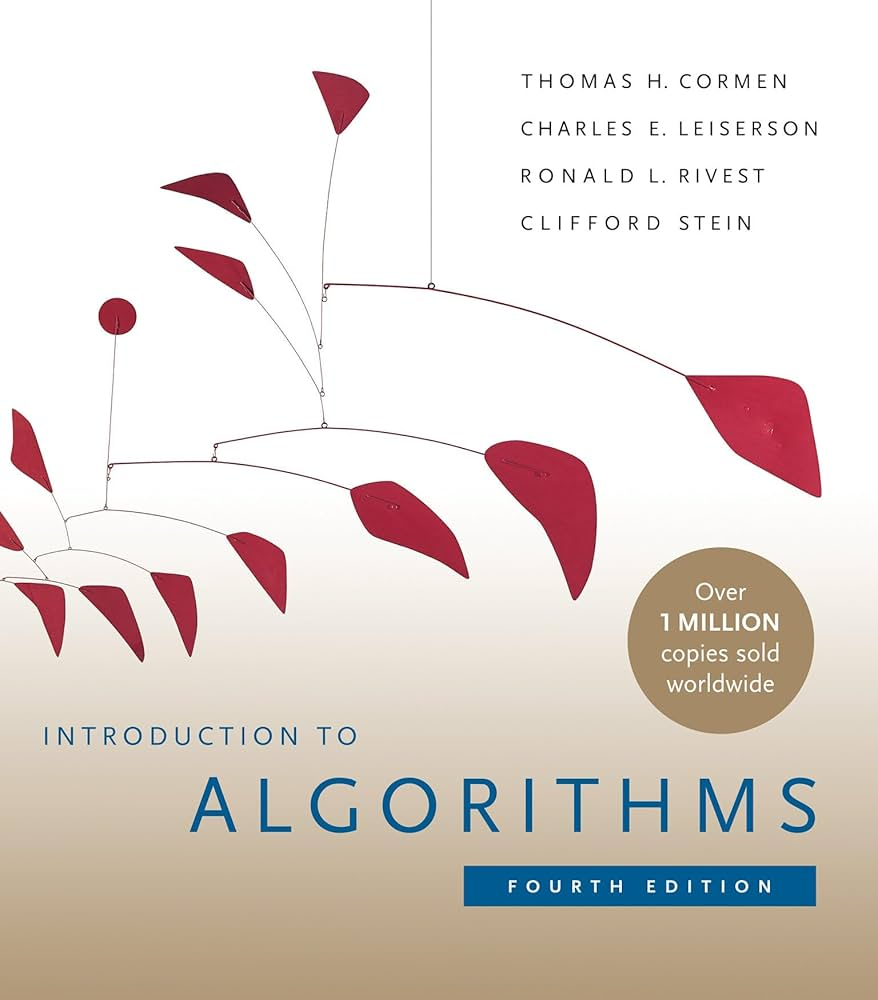
\includegraphics[width=0.45\textwidth]{figures/book_cover.jpg} \\
    \vspace{5mm}{
        \tiny
        Content has been extracted from \textit{Introduction to Algorithms}, Fourth Edition, by Cormen, Leiserson, Rivest, and Stein. MIT Press. 2022.\\
        Visit \url{https://mitpress.mit.edu/9780262046305/introduction-to-algorithms/}.\\
        Original slides from \textit{Introduction to Algorithms 6.046J/18.401J}, Fall 2005 Class by Prof. Charles Leiserson and Prof. Erik Demaine. MIT OpenCourseWare Initiative available at \url{https://ocw.mit.edu/courses/6-046j-introduction-to-algorithms-sma-5503-fall-2005/}.\\
    }
\end{frame}

\section{Quicksort}

\begin{frame}{Quicksort}
    \begin{itemize}
            \item Proposed by C.A.R. Hoare in 1962.
            \item Divide-and-conquer algorithm.
            \item Sorts `in place' (like insertion sort, but not like merge sort).
            \item Very practical (with tuning).
    \end{itemize}
\end{frame}

\section{Divide \& Conquer}

\begin{frame}{Divide and Conquer}
    Quicksort an $n$-element array:
    \begin{enumerate}
        \item \textbf{\Large Divide:} Partition the array into two subarrays around a \textbf{pivot} $x$ such that elements in lower subarray $\leq x \leq$ elements in upper subarray.
            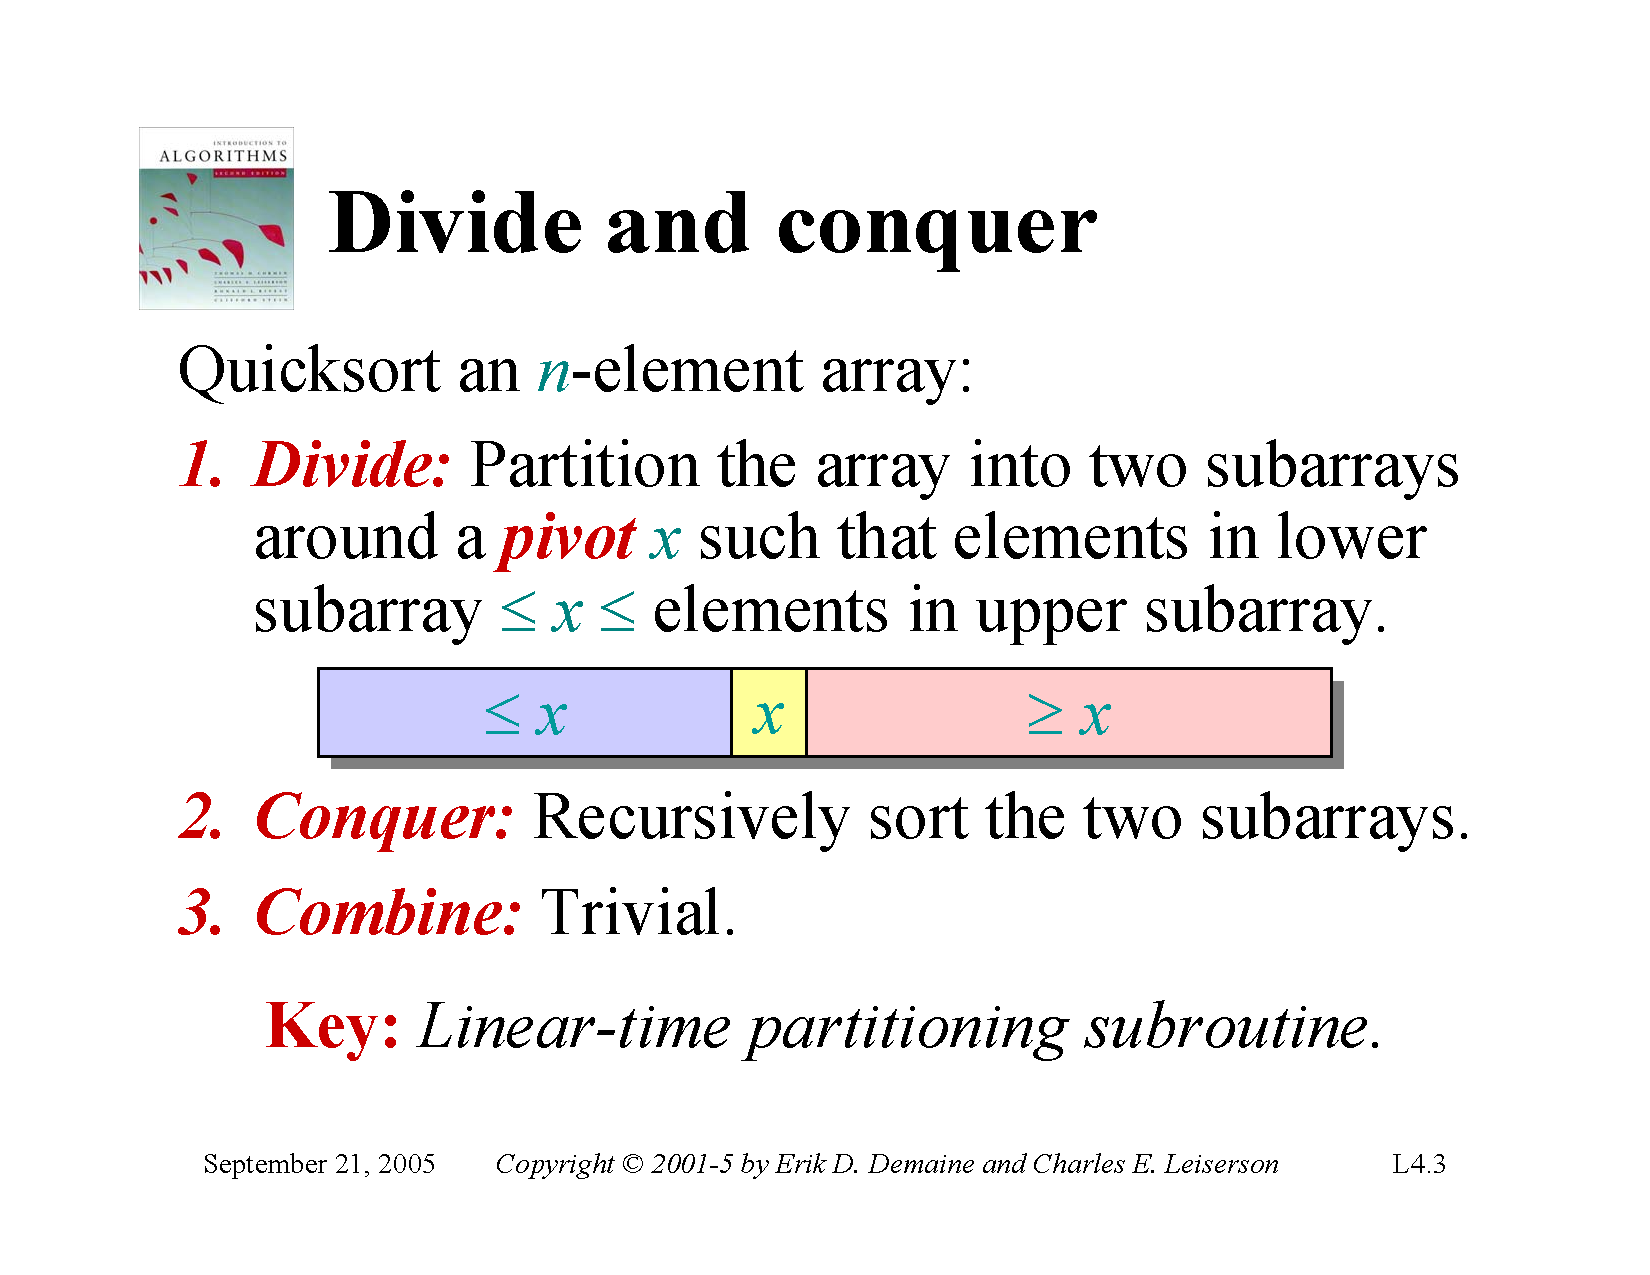
\includegraphics[width=\textwidth, trim={2cm 7.25cm 2cm 9.75cm}, clip]{pages/lec4_3} 
        \item \textbf{\Large Conquer:} Recursively sort the two subarrays.
        \item \textbf{\Large Combine:} Trivial.
    \end{enumerate}
    \begin{alertblock}{Key:}
        Linear-time partitioning subroutine.
    \end{alertblock}
\end{frame}

\section{Partitioning}

\begin{frame}{Partitioning Subroutine}
    \begin{minipage}{0.58\textwidth}
        \begin{algorithm}[H]
            \begin{algorithmic}[1]
                %\State \hrulefill
                \Procedure{\textsc{Partition}}{$A$, $p$, $q$}
                    \State $x \leftarrow A[p]$
                    \State $i \leftarrow p$
                    \For{$j \leftarrow p + 1$ \textbf{to} $q$}
                        \If{$A[j] \leq x$}
                            \State $i \leftarrow i + 1$
                            \State exchange $A[i] \leftrightarrow A[j]$
                        \EndIf
                    \EndFor
                    \State exchange $A[p] \leftrightarrow A[i]$
                    \State \Return $i$
                \EndProcedure
            \end{algorithmic}
        \end{algorithm}
    \end{minipage}
    \hfill
    \begin{minipage}{0.38\textwidth}
        \begin{alertblock}{Running time:}
            $O(n)$ for $n$ elements.
        \end{alertblock}
        \vspace{4.5cm}
    \end{minipage}
    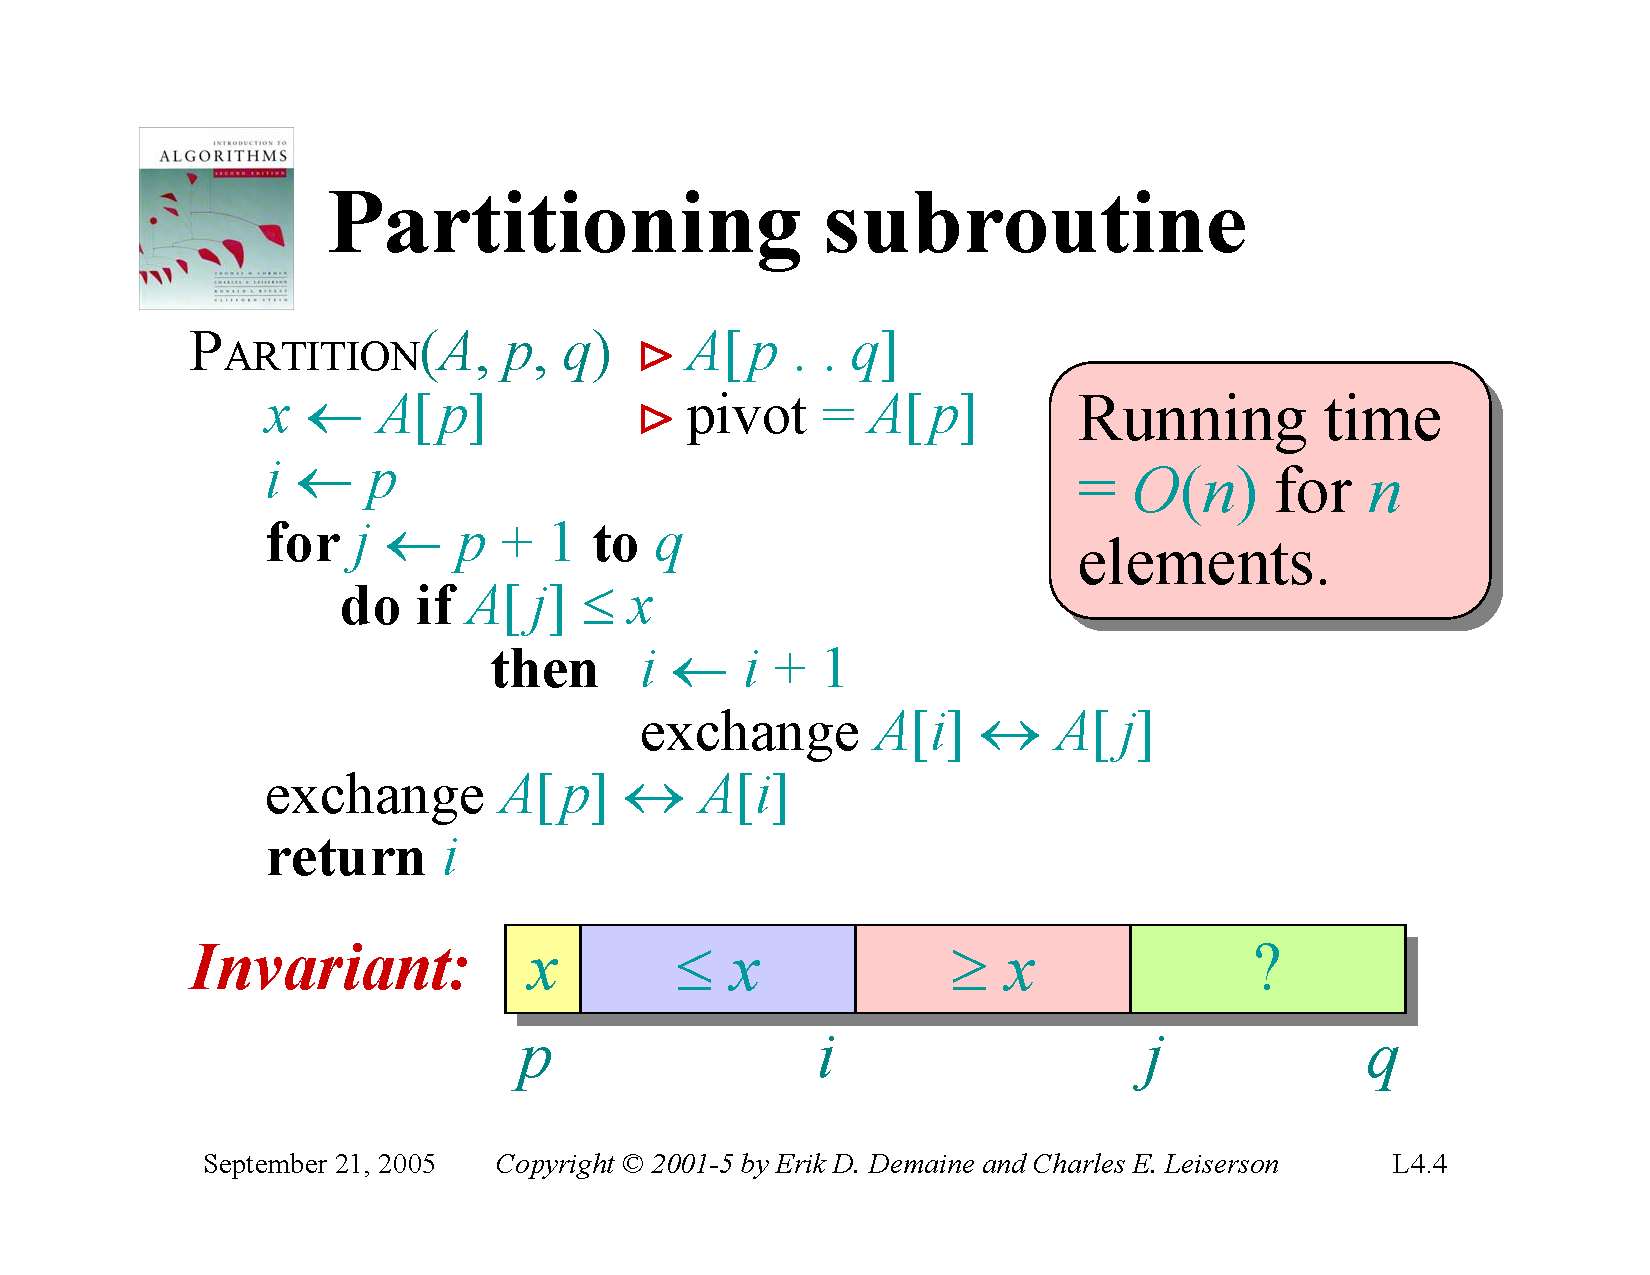
\includegraphics[width=\textwidth, trim={1.75cm 1.50cm 2.50cm 14.30cm}, clip]{pages/lec4_4} 
\end{frame}

\begin{frame}{Example of partitioning}
    \centering
    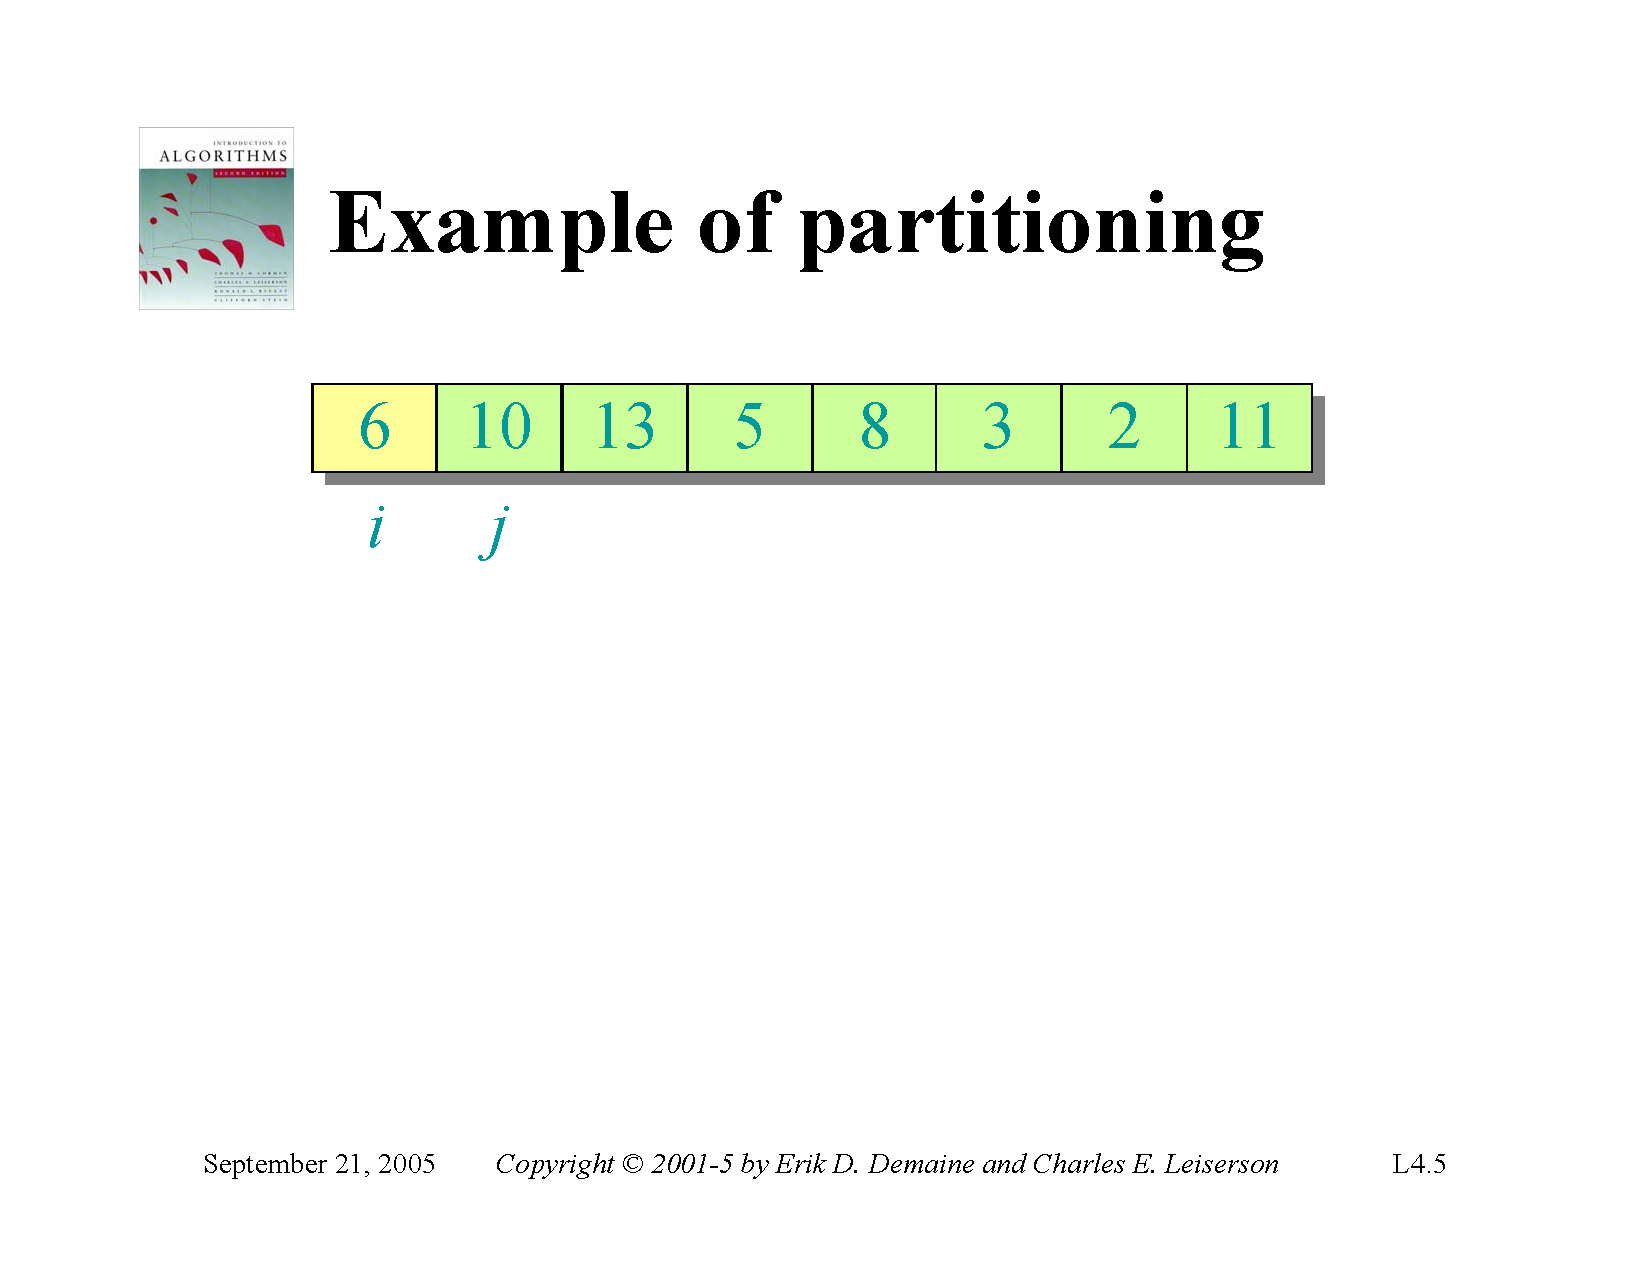
\includegraphics[width=\textwidth, trim={2.75cm 1.80cm 2.75cm 5.00cm}, clip]{pages/lec4_5}
\end{frame}
\begin{frame}{Example of partitioning}
    \centering
    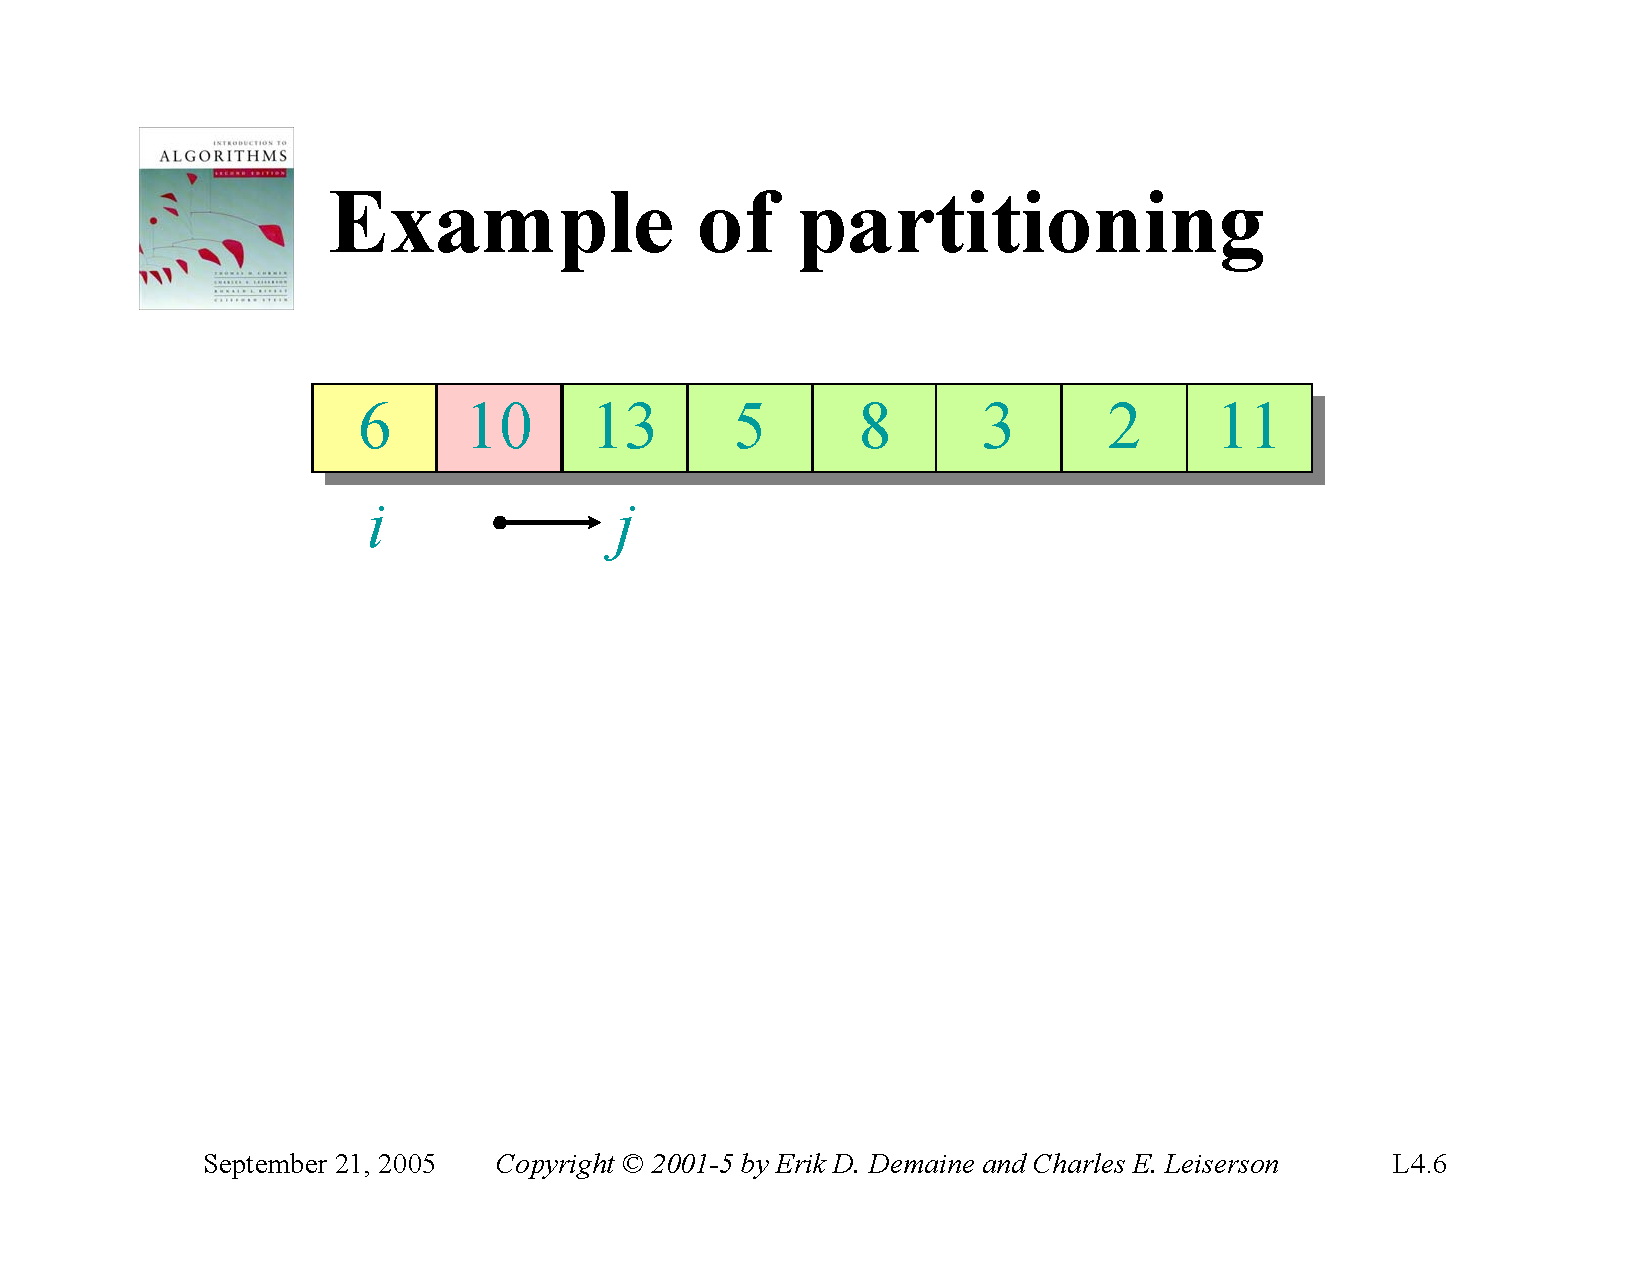
\includegraphics[width=\textwidth, trim={2.75cm 1.80cm 2.75cm 5.00cm}, clip]{pages/lec4_6}
\end{frame}
\begin{frame}{Example of partitioning}
    \centering
    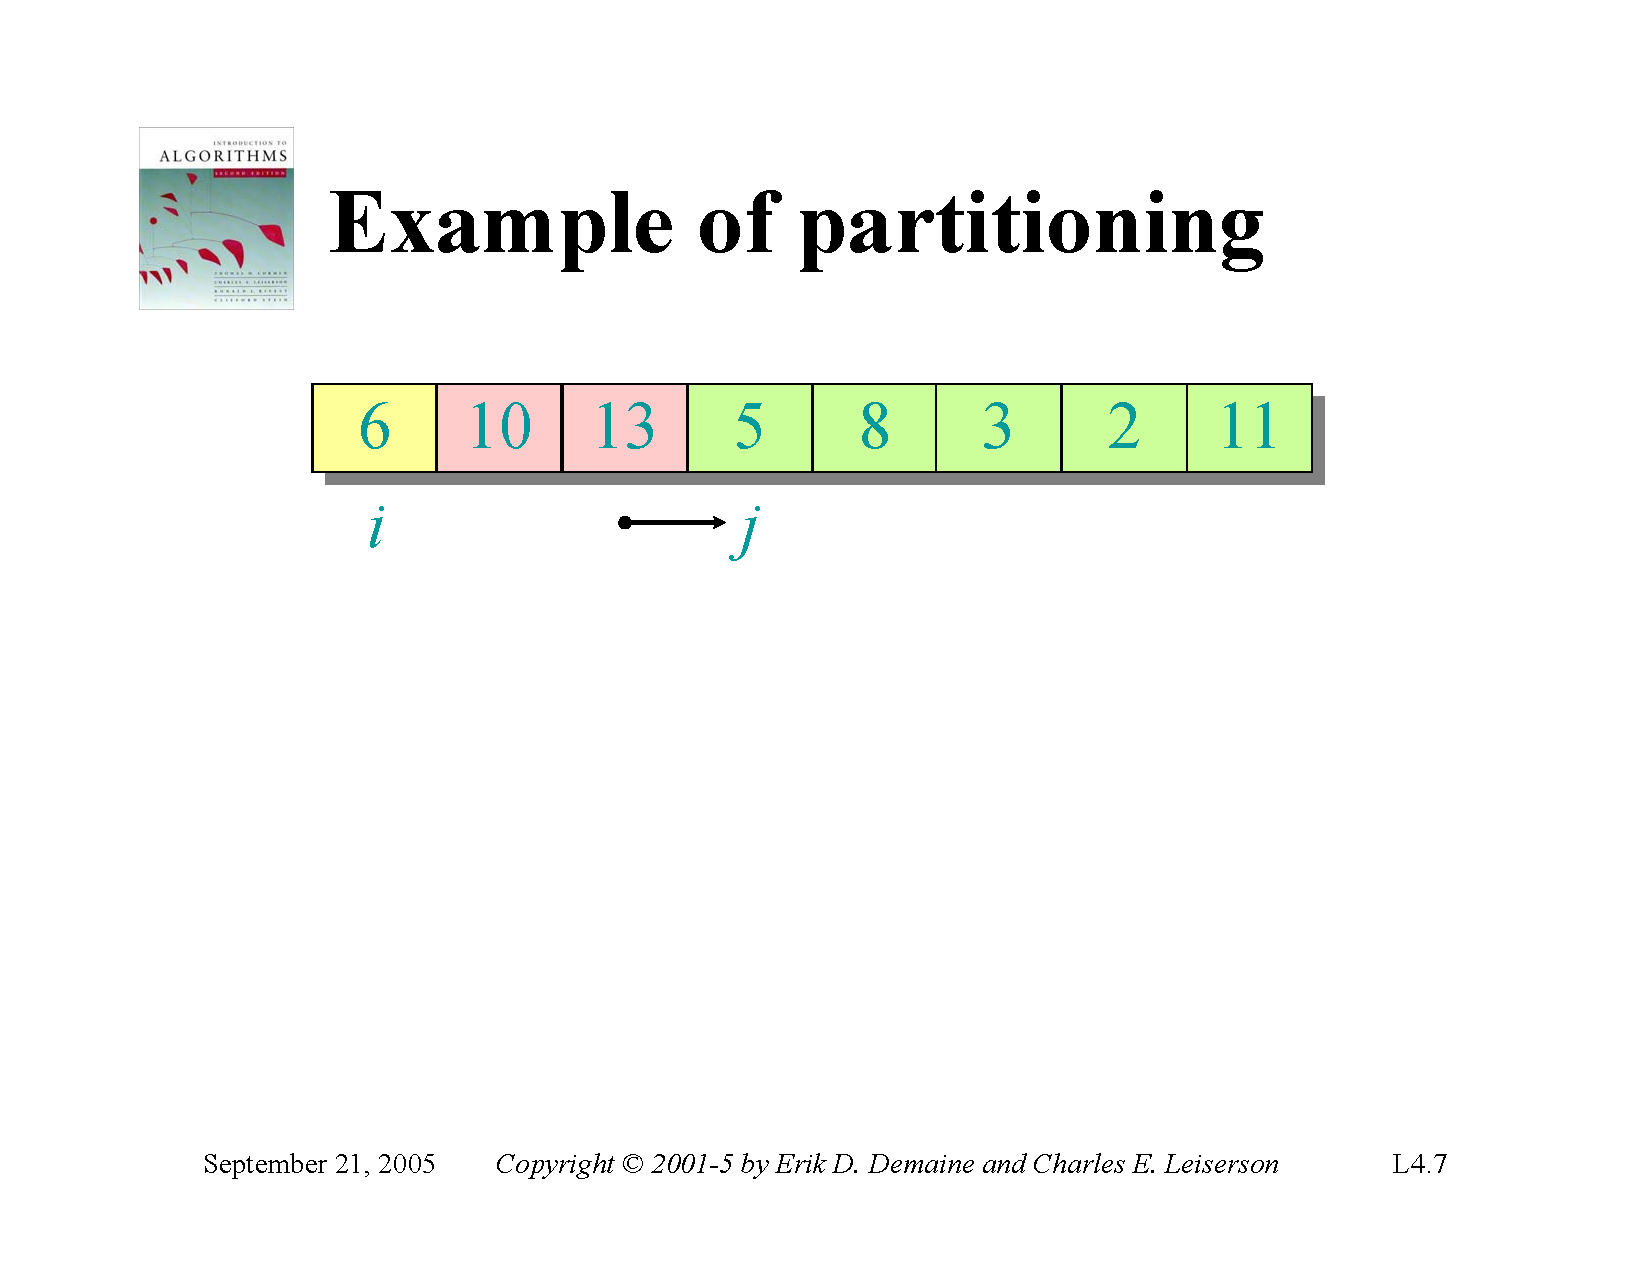
\includegraphics[width=\textwidth, trim={2.75cm 1.80cm 2.75cm 5.00cm}, clip]{pages/lec4_7}
\end{frame}
\begin{frame}{Example of partitioning}
    \centering
    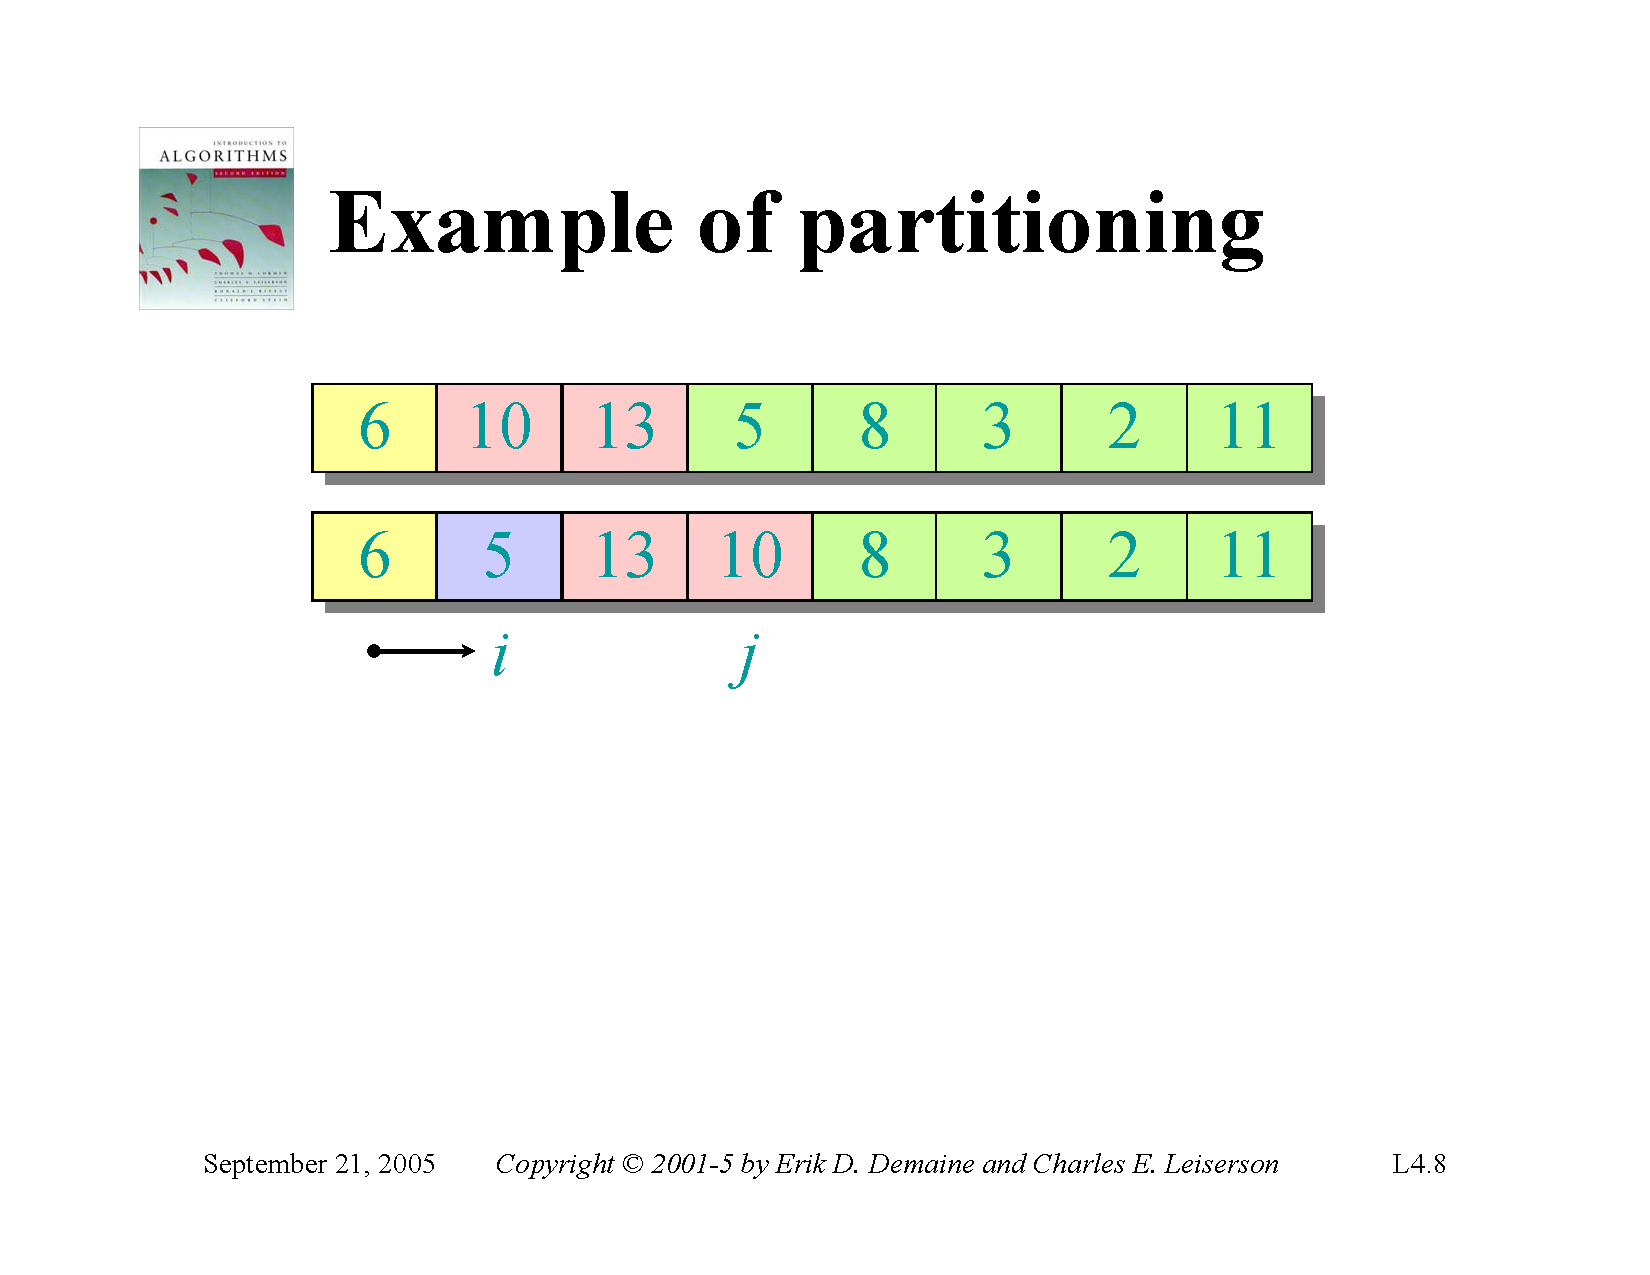
\includegraphics[width=\textwidth, trim={2.75cm 1.80cm 2.75cm 5.00cm}, clip]{pages/lec4_8}
\end{frame}
\begin{frame}{Example of partitioning}
    \centering
    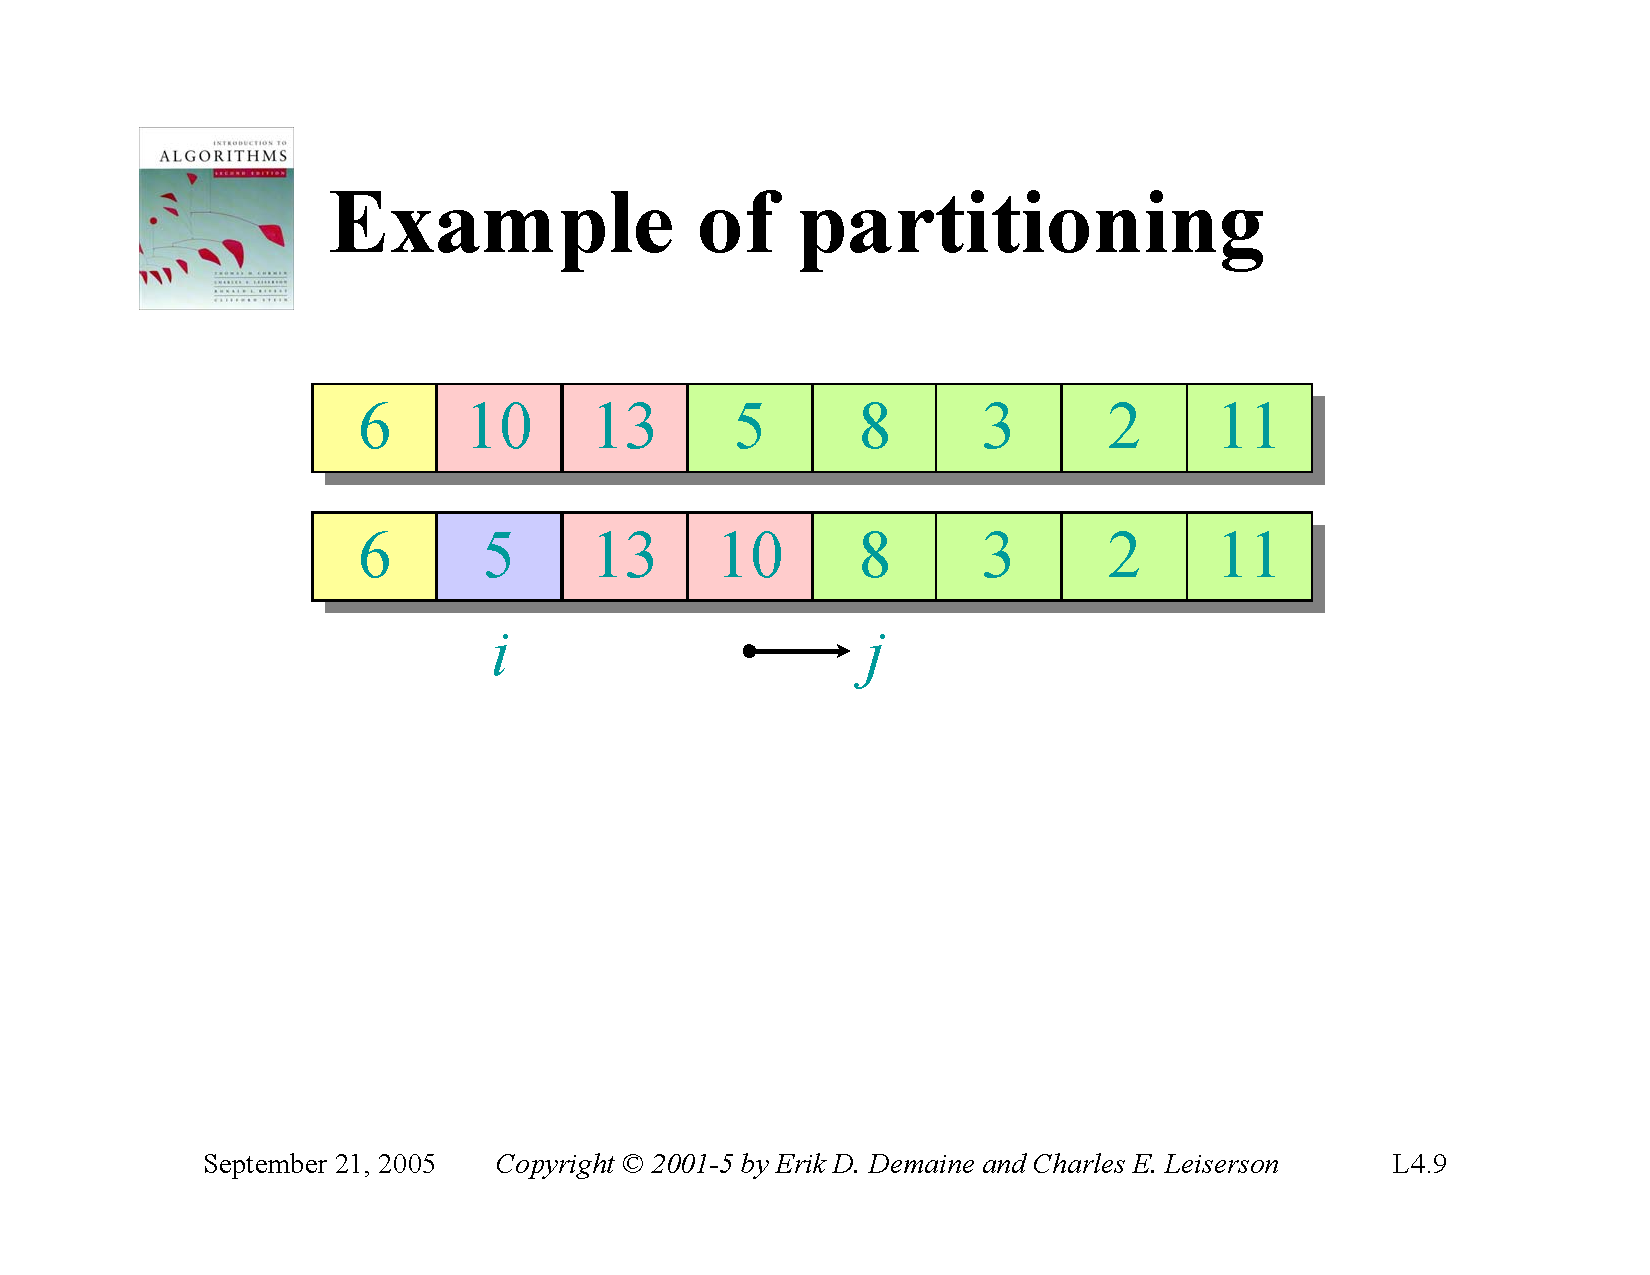
\includegraphics[width=\textwidth, trim={2.75cm 1.80cm 2.75cm 5.00cm}, clip]{pages/lec4_9}
\end{frame}
\begin{frame}{Example of partitioning}
    \centering
    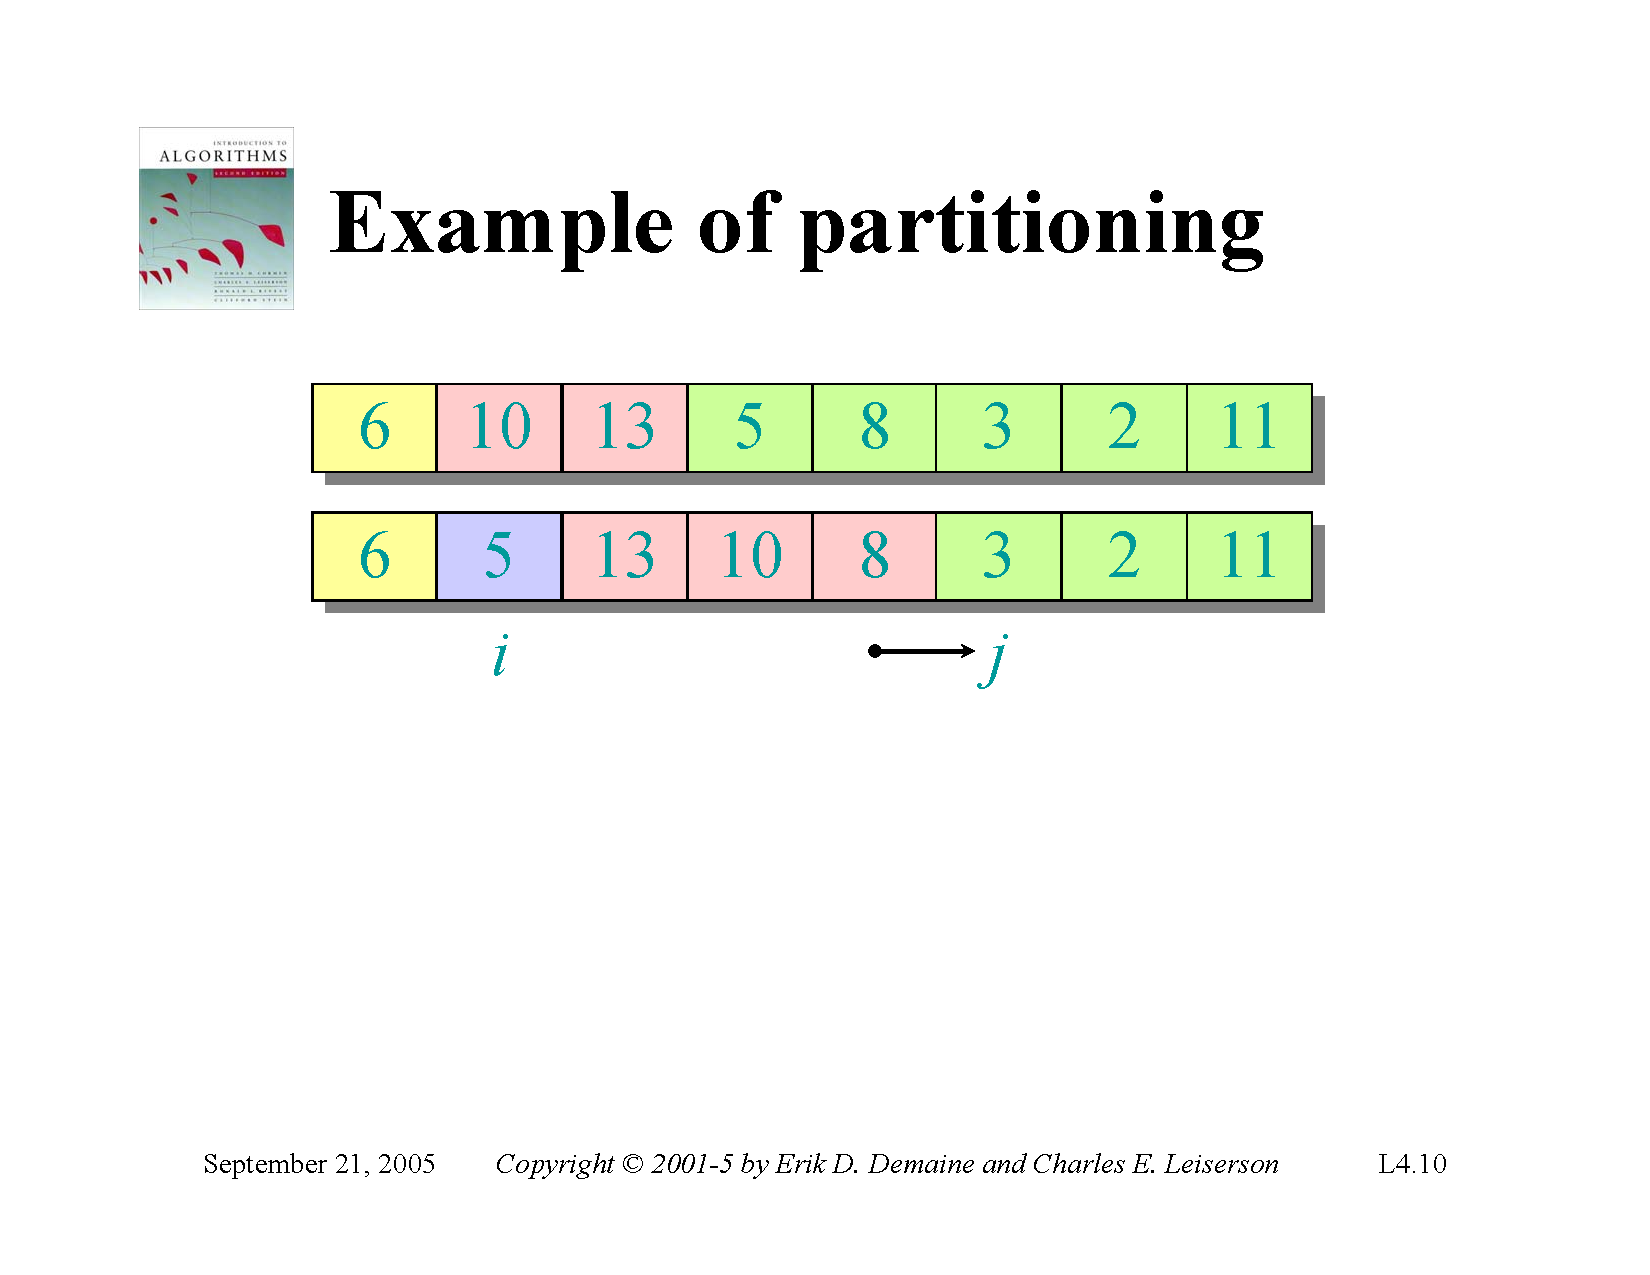
\includegraphics[width=\textwidth, trim={2.75cm 1.80cm 2.75cm 5.00cm}, clip]{pages/lec4_10}
\end{frame}
\begin{frame}{Example of partitioning}
    \centering
    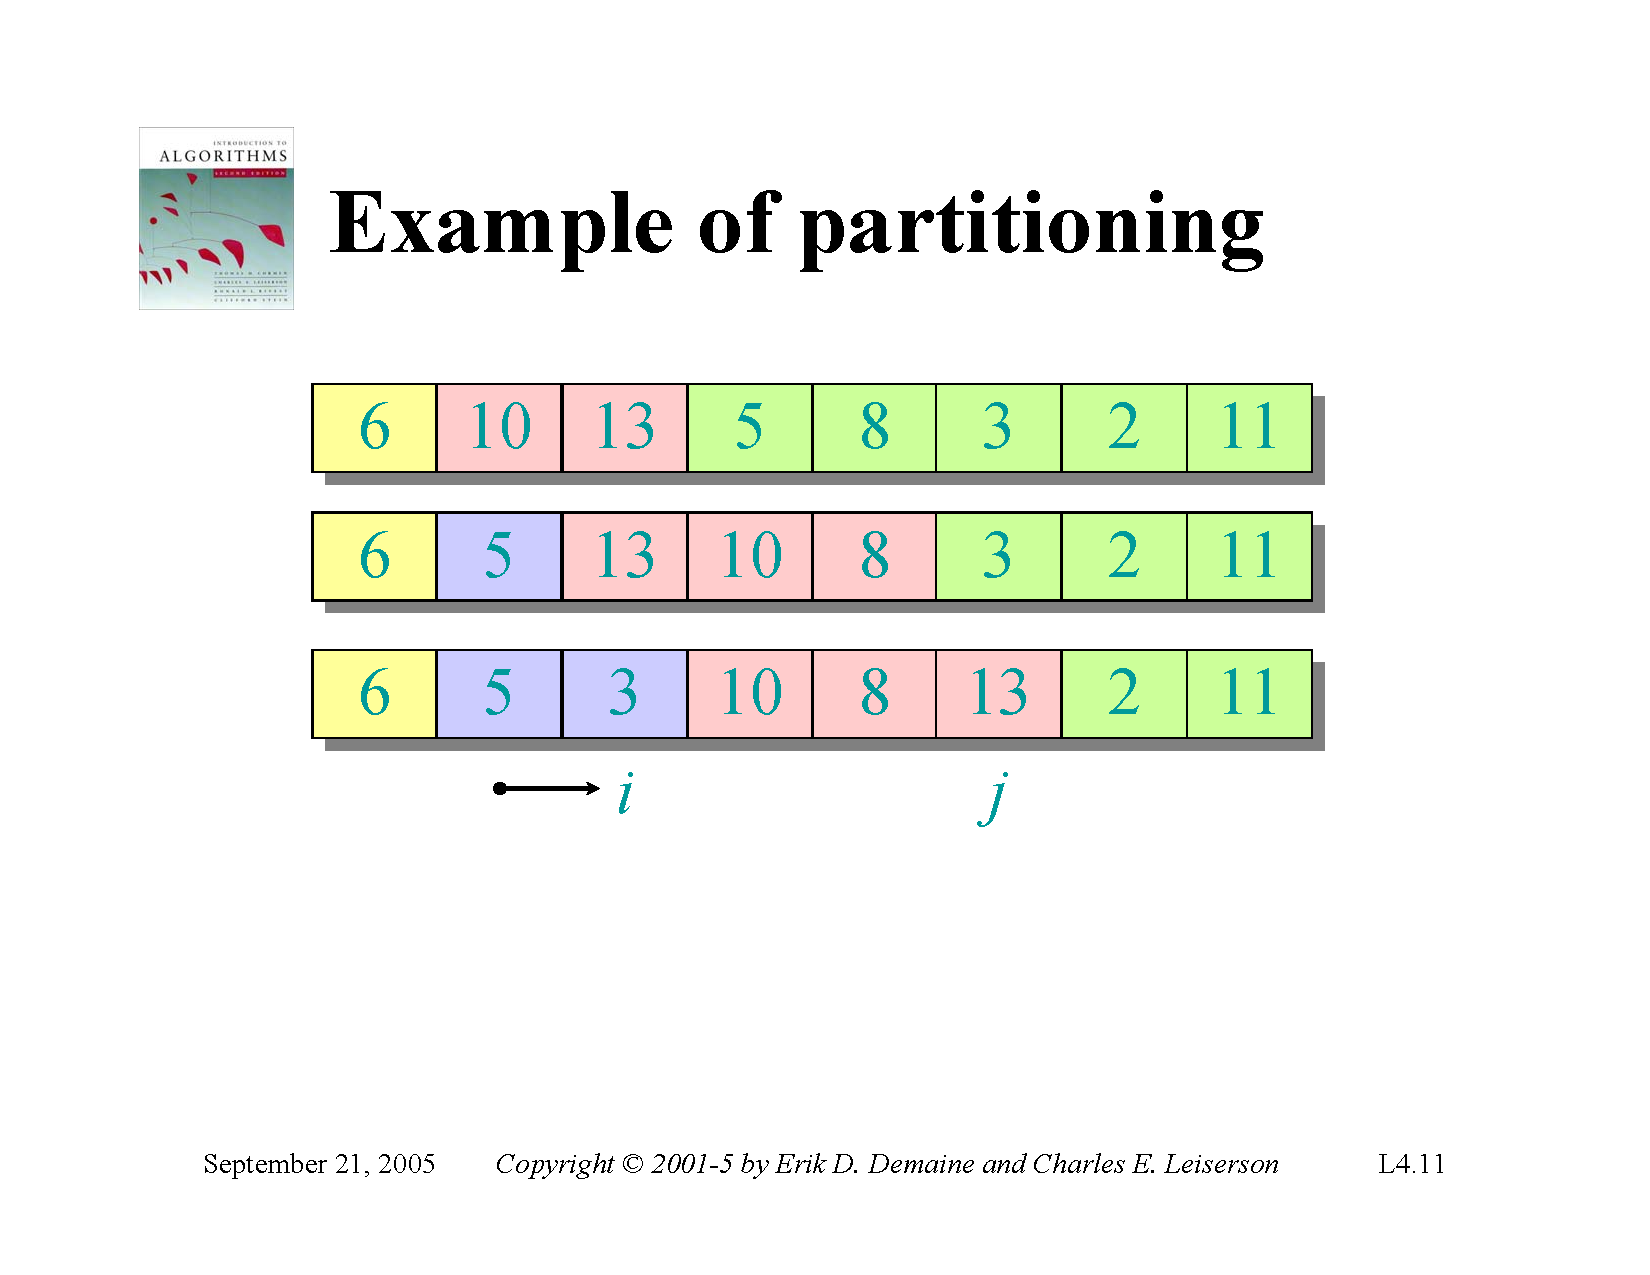
\includegraphics[width=\textwidth, trim={2.75cm 1.80cm 2.75cm 5.00cm}, clip]{pages/lec4_11}
\end{frame}
\begin{frame}{Example of partitioning}
    \centering
    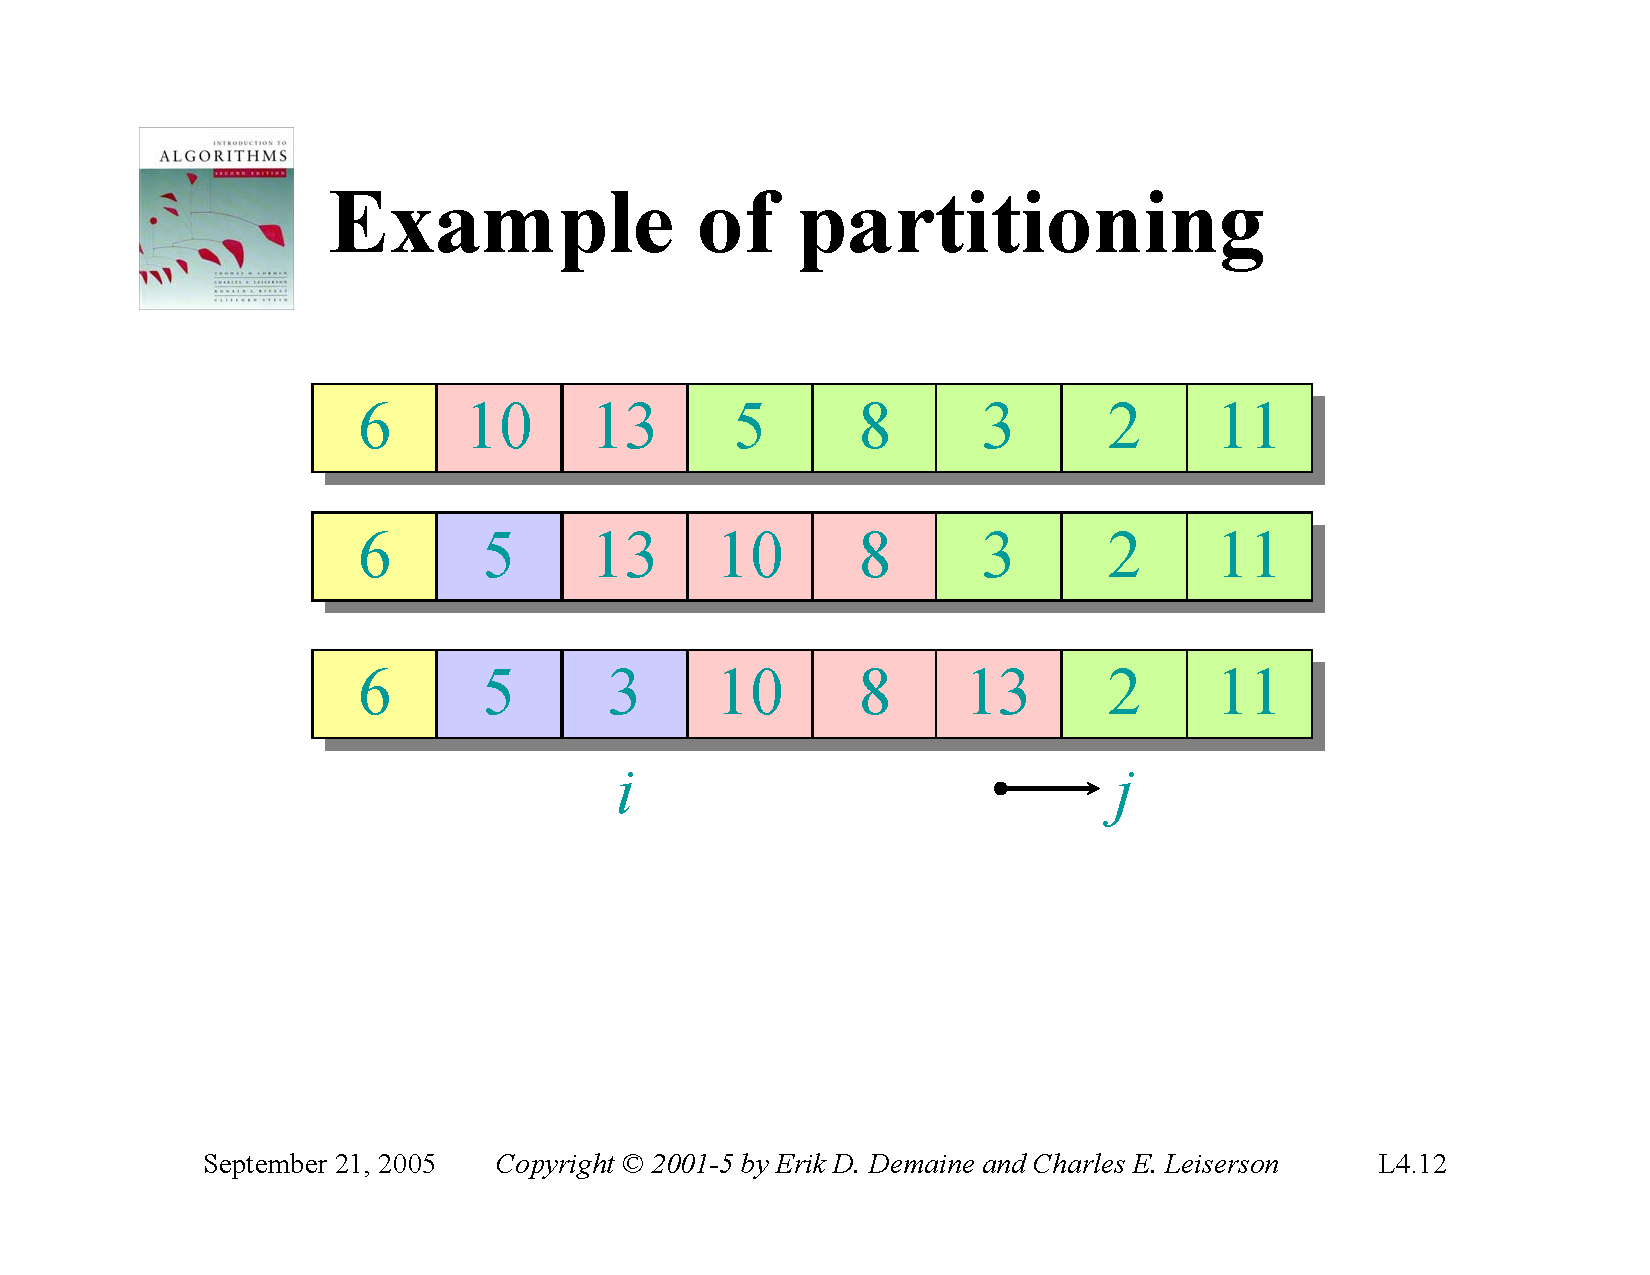
\includegraphics[width=\textwidth, trim={2.75cm 1.80cm 2.75cm 5.00cm}, clip]{pages/lec4_12}
\end{frame}
\begin{frame}{Example of partitioning}
    \centering
    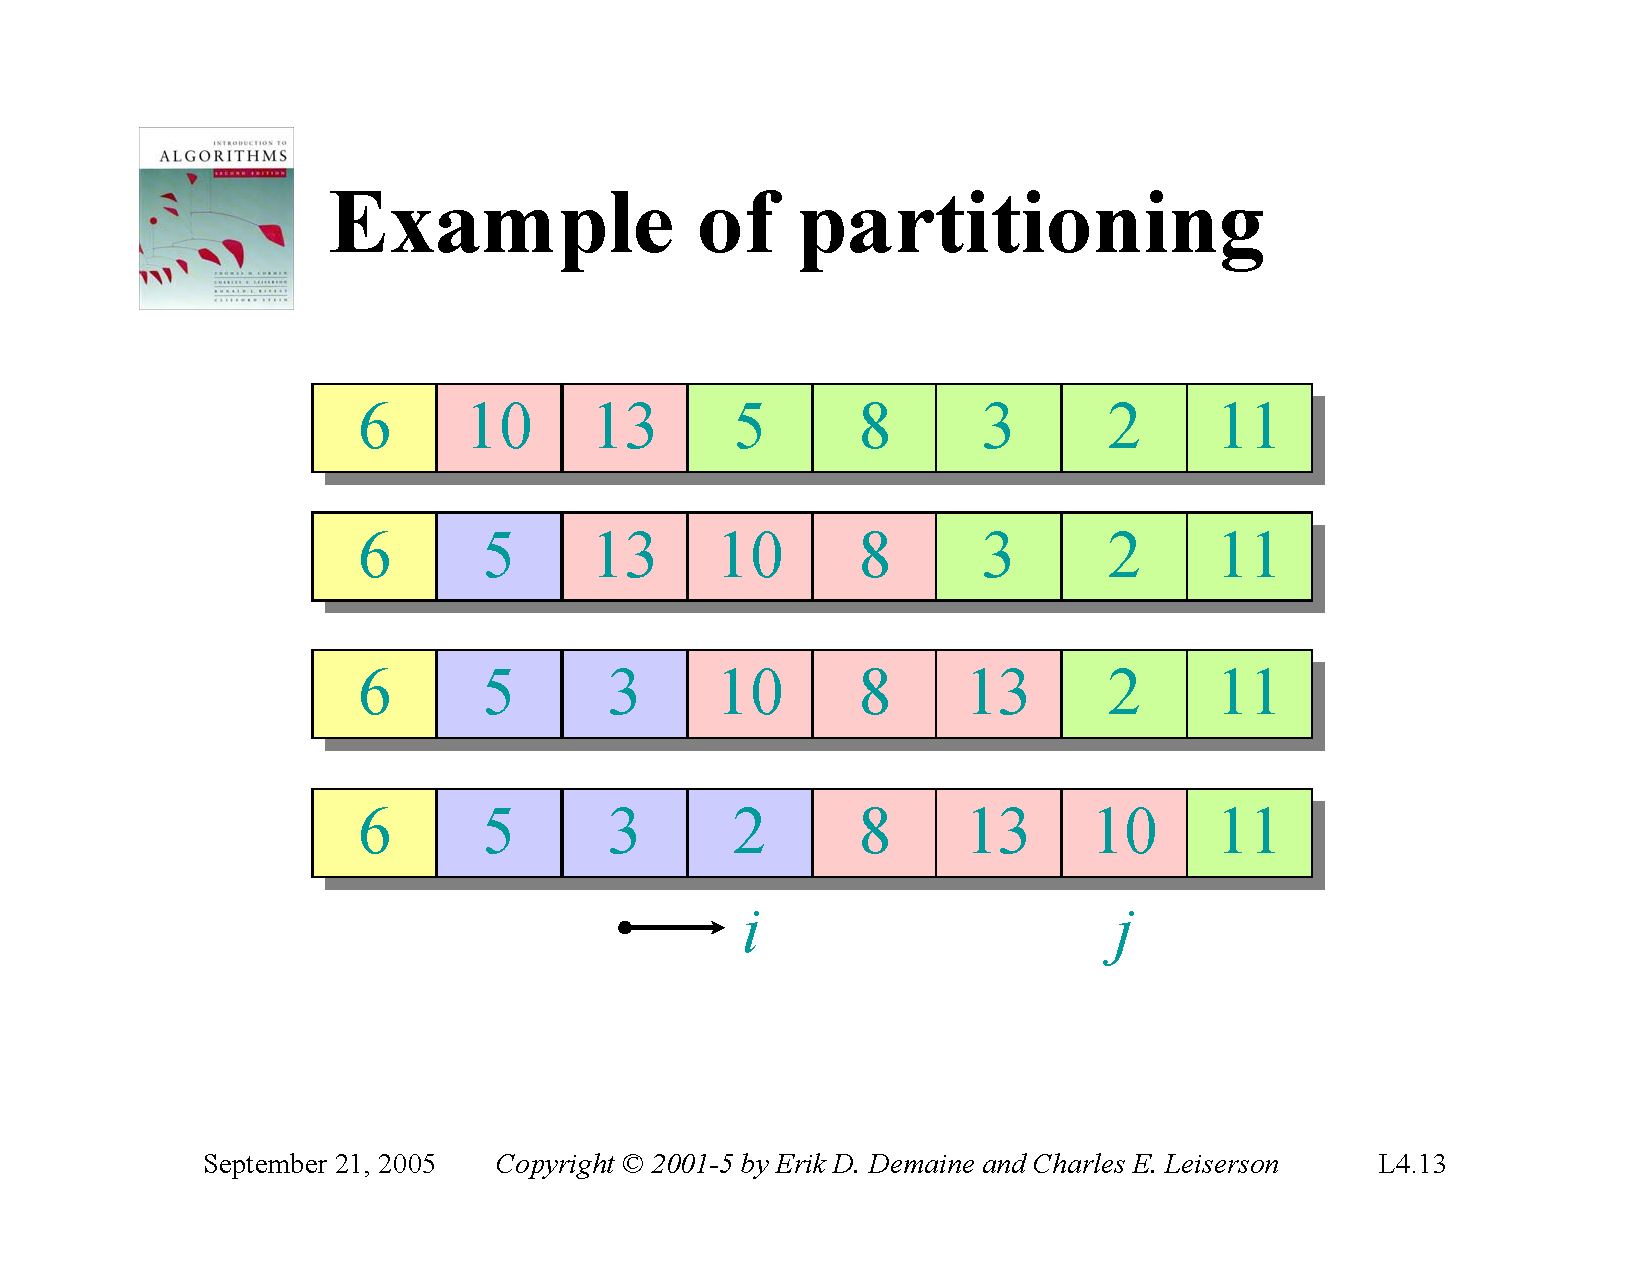
\includegraphics[width=\textwidth, trim={2.75cm 1.80cm 2.75cm 5.00cm}, clip]{pages/lec4_13}
\end{frame}
\begin{frame}{Example of partitioning}
    \centering
    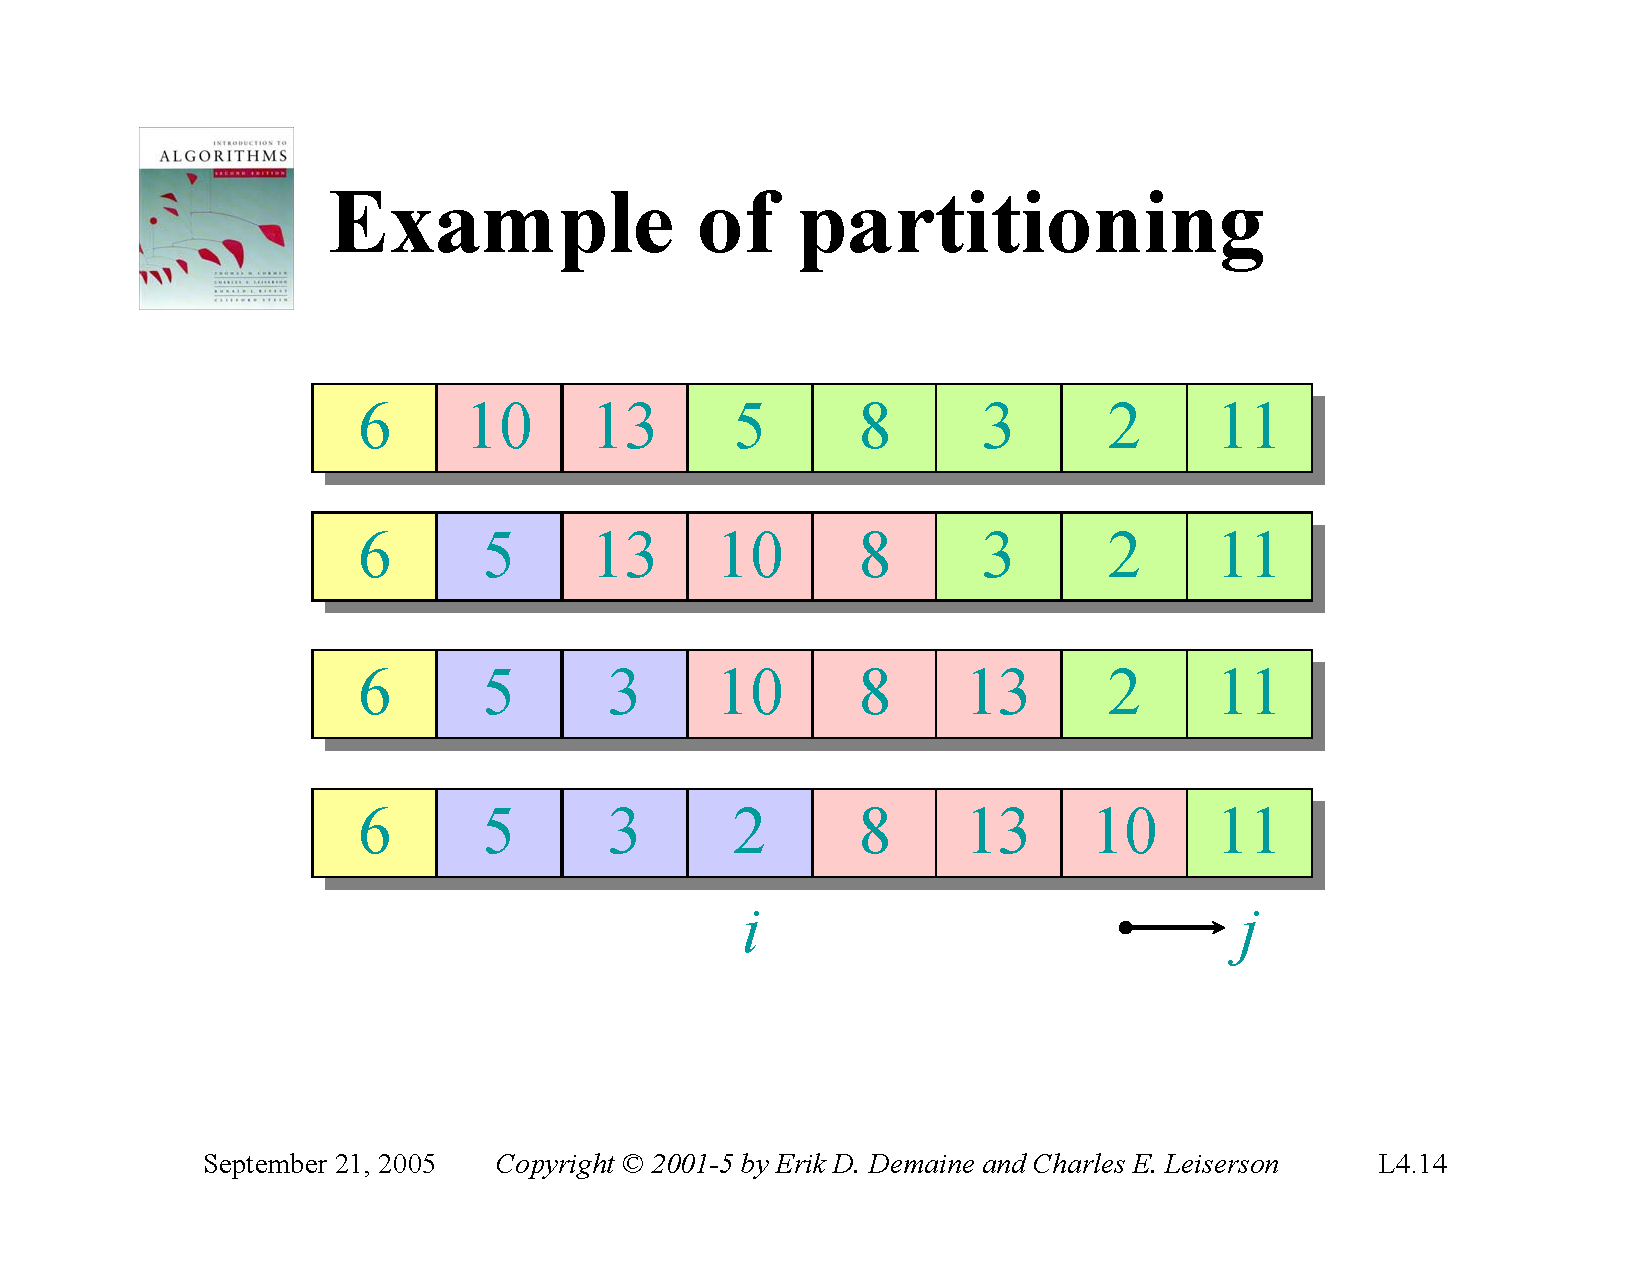
\includegraphics[width=\textwidth, trim={2.75cm 1.80cm 2.75cm 5.00cm}, clip]{pages/lec4_14}
\end{frame}
\begin{frame}{Example of partitioning}
    \centering
    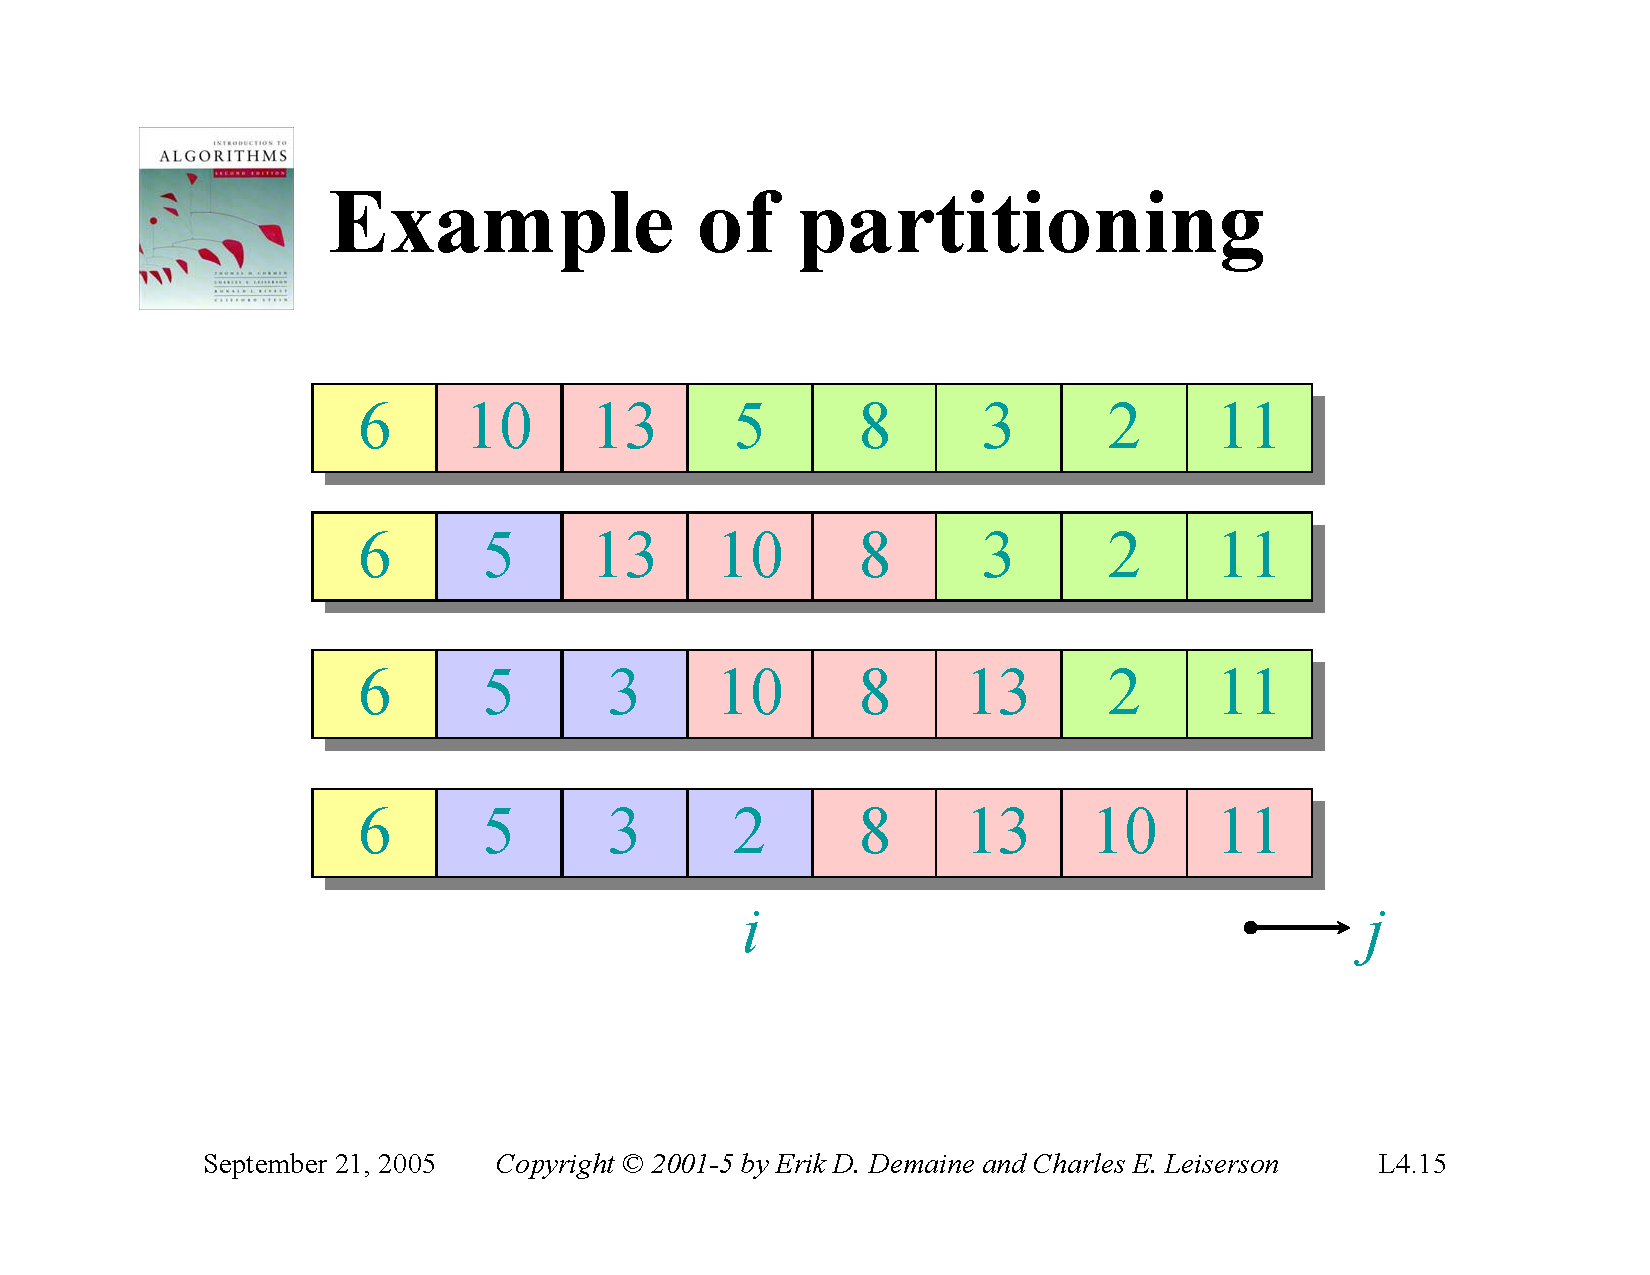
\includegraphics[width=\textwidth, trim={2.75cm 1.80cm 2.75cm 5.00cm}, clip]{pages/lec4_15}
\end{frame}
\begin{frame}{Example of partitioning}
    \centering
    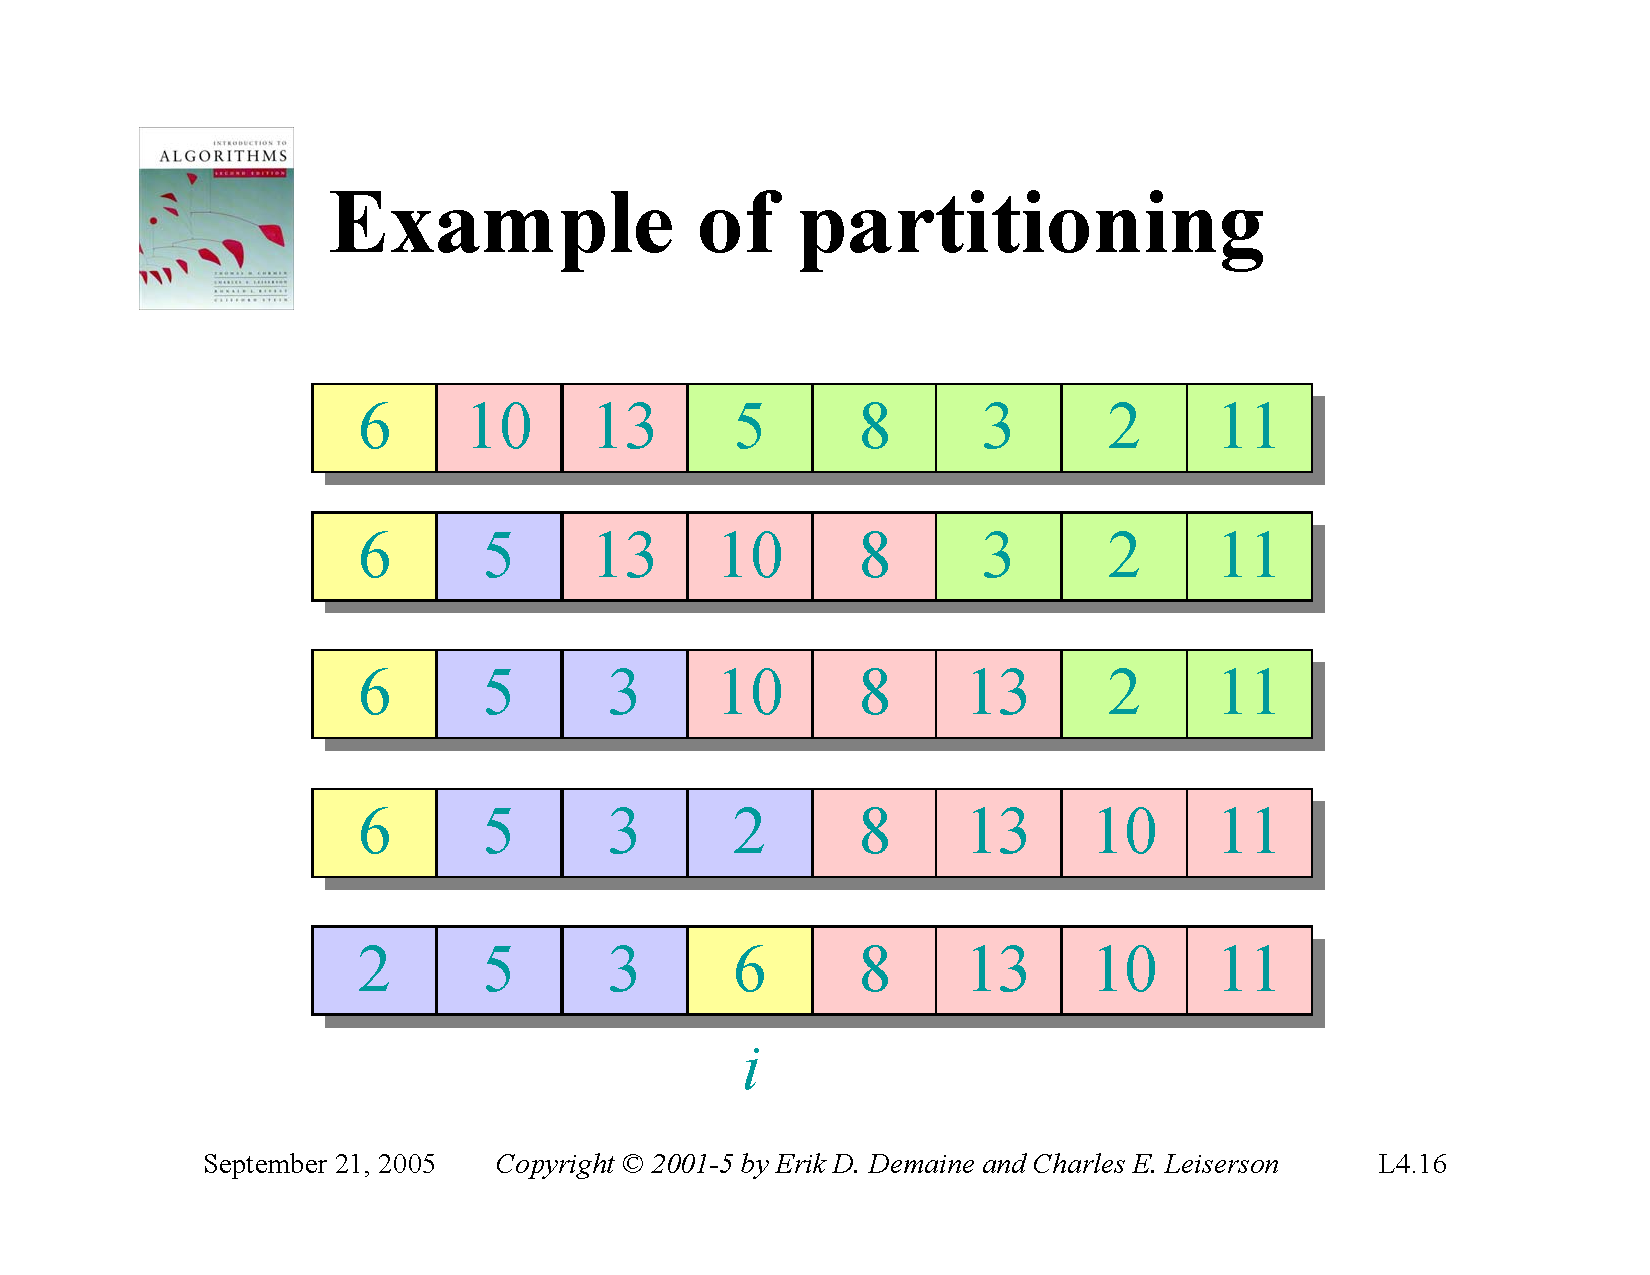
\includegraphics[width=\textwidth, trim={2.75cm 1.80cm 2.75cm 5.00cm}, clip]{pages/lec4_16}
\end{frame}

\begin{frame}{Pseudocode for Quicksort}
        \begin{algorithm}[H]
            \begin{algorithmic}[1]
                \Procedure{\textsc{Quicksort}}{$A$, $p$, $r$}
                    \If{$p < r$}
                        \State $q \leftarrow$ \textsc{Partition}($A$,$p$, $r$)
                        \State \textsc{Quicksort}($A$, $p$, $q - 1$)
                        \State \textsc{Quicksort}($A$, $q + 1$, $r$)
                    \EndIf
                \EndProcedure
            \end{algorithmic}
        \end{algorithm}
        \begin{alertblock}{Initial call:}
            \textsc{Quicksort}($A$, $1$, $n$)
        \end{alertblock}
\end{frame}

\begin{frame}{Analysis of Quicksort}
    \begin{itemize}
        \item Assume all input elements are distinct.
        \item In practice, there are better partitioning algorithms for when duplicate input elements may exist.
        \item Let $T(n) =$ worst-case running time on an array of $n$ elements.
    \end{itemize}
\end{frame}

\section{Worst-case Analysis}

\begin{frame}{Worst-case of Quicksort}
    \begin{itemize}
        \item Input sorted or reverse sorted.
        \item Partition around min or max element.
        \item One side of partition always has no elements.
    \end{itemize}
    \begin{equation*}
        \begin{split}
            T(n) =& T(0) + T(n - 1) + \Theta(n) \\
                    =& \Theta(1) + T(n - 1) + \Theta(n) \\
                    =& T(n - 1) + \Theta(n) \\
                    =& \Theta(n^2)
        \end{split}
    \end{equation*}
    \pause
    \centering
    \textcolor{red}{\textbf{Arithmetic Series!}}
\end{frame}

\begin{frame}{Worst-case Recursion Tree}
    \begin{equation*}
        \begin{split}
            T(n) =& T(0) + T(n - 1) + cn \\
        \end{split}
    \end{equation*}
    \centering
    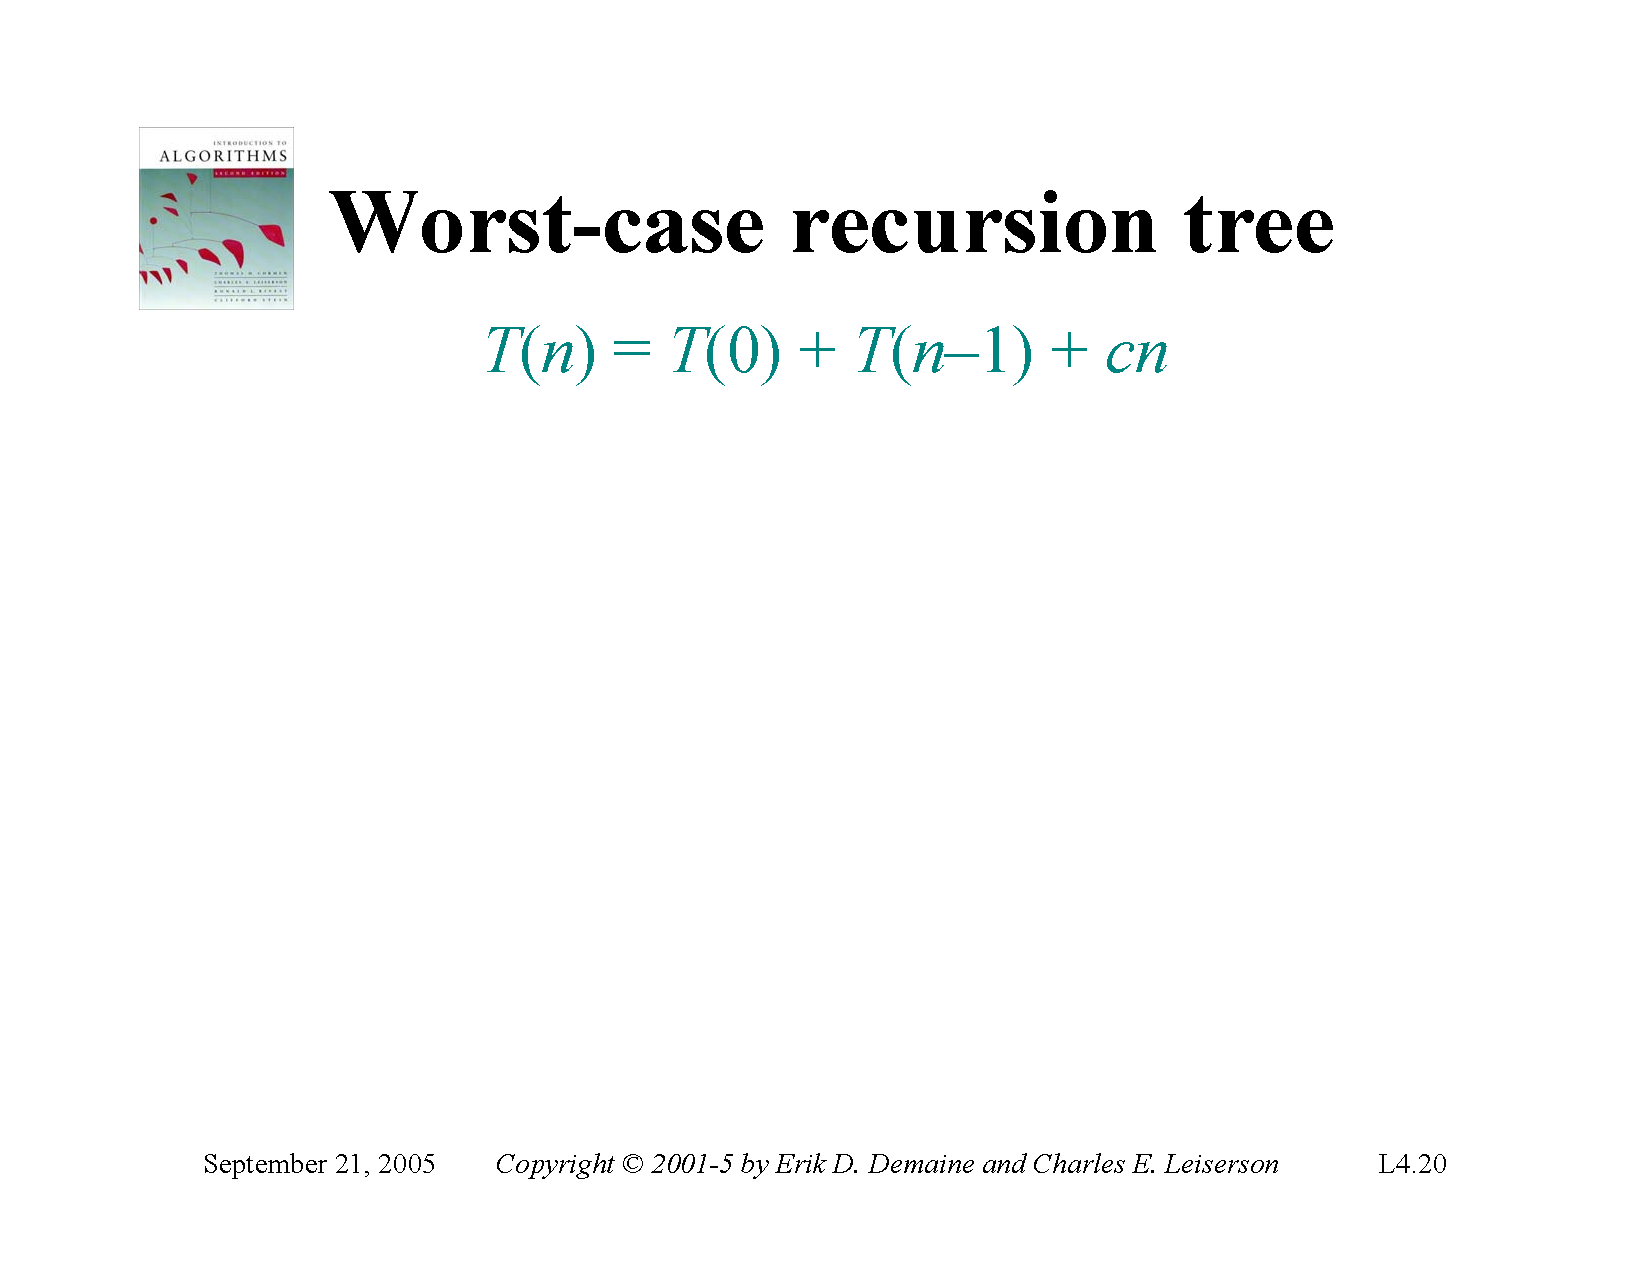
\includegraphics[width=\textwidth, trim={1.00cm 1.80cm 0.50cm 5.25cm}, clip]{pages/lec4_20}
\end{frame}

\begin{frame}{Worst-case Recursion Tree}
    \begin{equation*}
        \begin{split}
            T(n) =& T(0) + T(n - 1) + cn \\
        \end{split}
    \end{equation*}
    \centering
    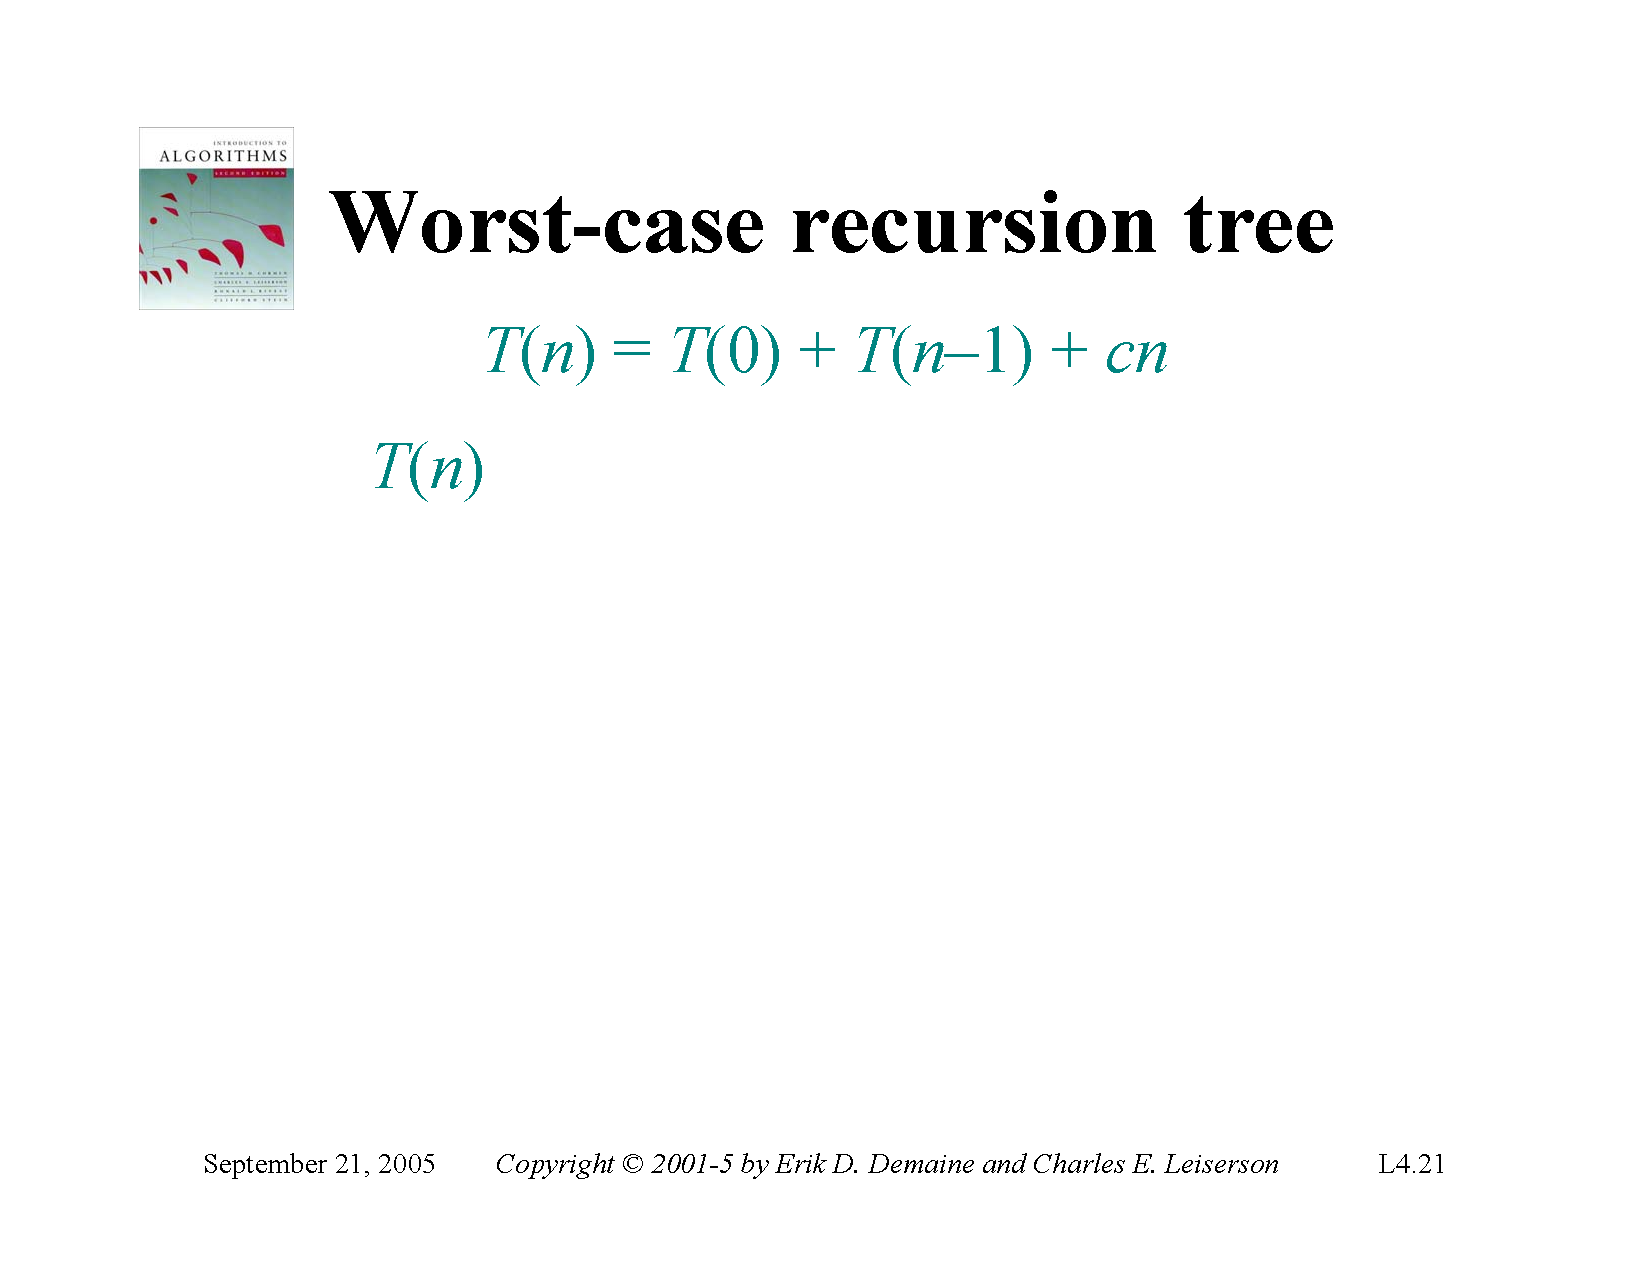
\includegraphics[width=\textwidth, trim={1.00cm 1.80cm 0.50cm 5.25cm}, clip]{pages/lec4_21}
\end{frame}
\begin{frame}{Worst-case Recursion Tree}
    \begin{equation*}
        \begin{split}
            T(n) =& T(0) + T(n - 1) + cn \\
        \end{split}
    \end{equation*}
    \centering
    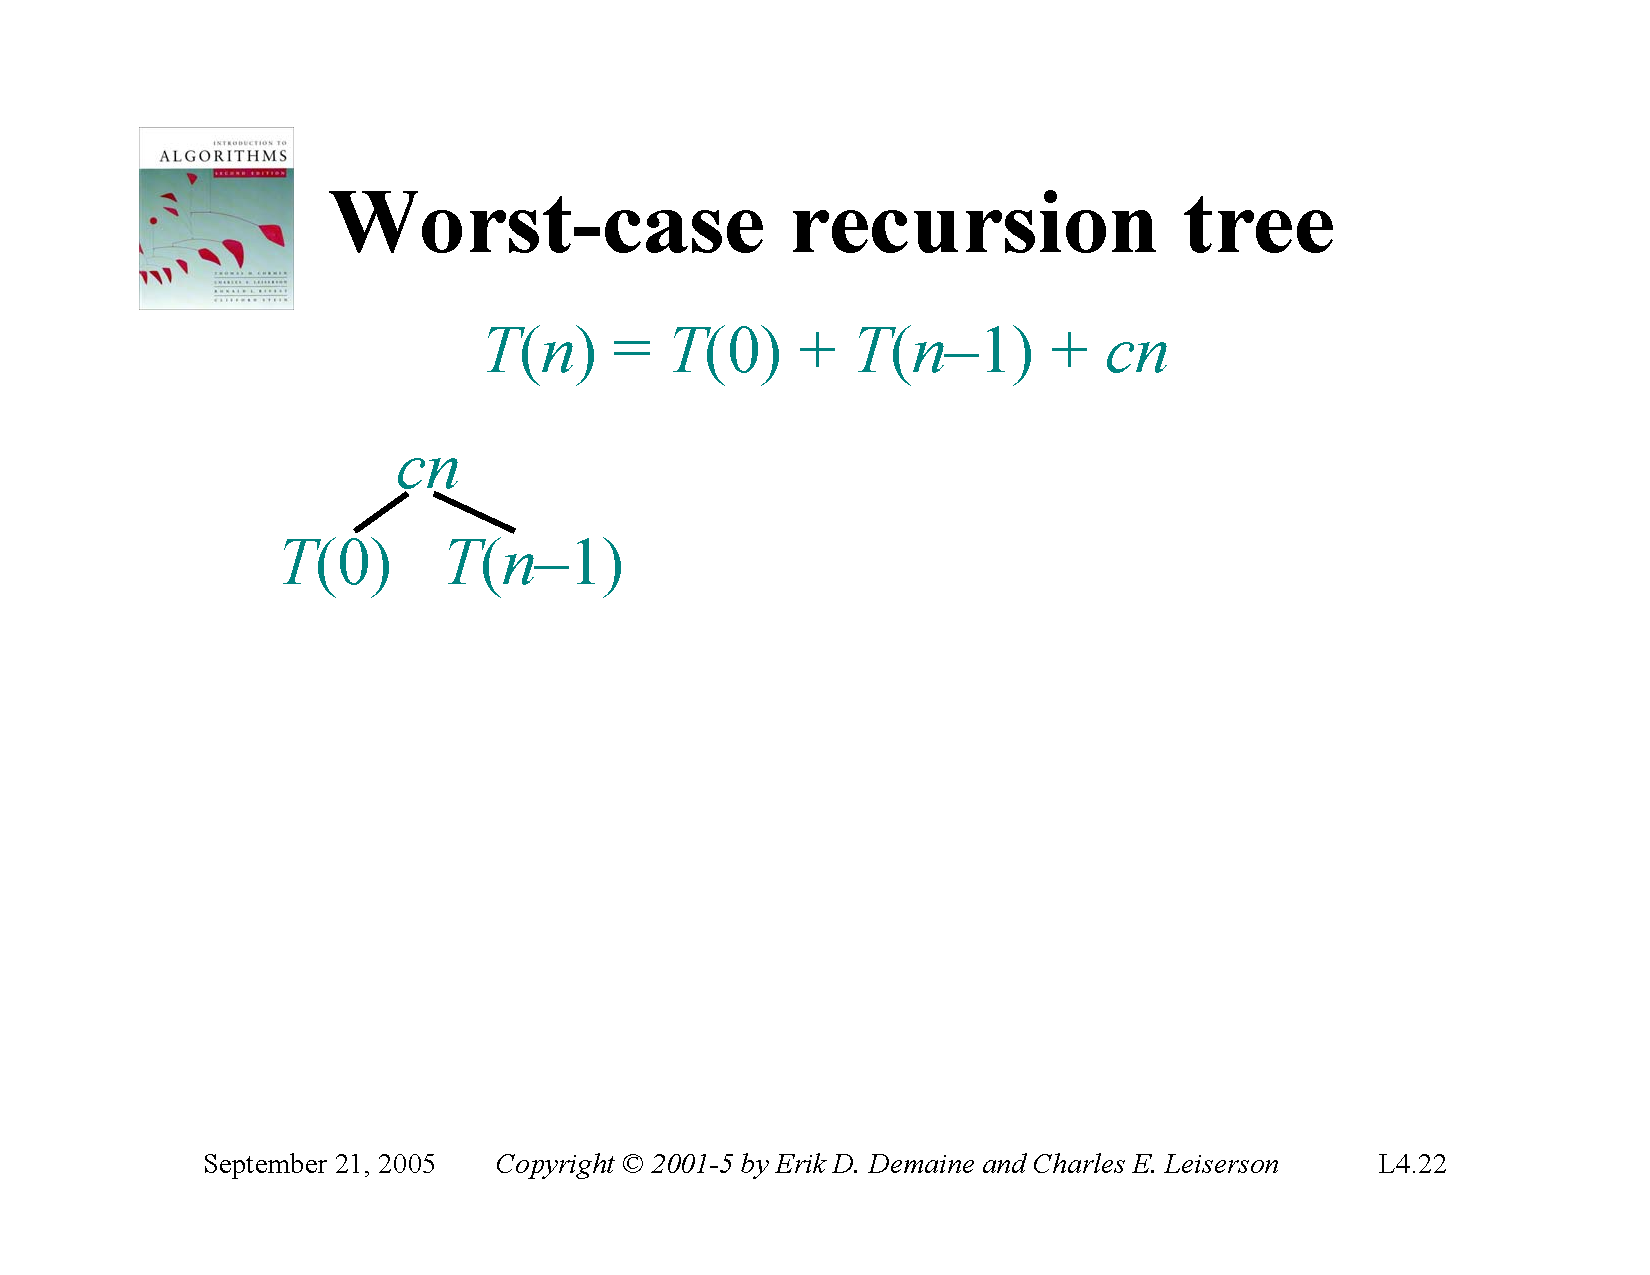
\includegraphics[width=\textwidth, trim={1.00cm 1.80cm 0.50cm 5.25cm}, clip]{pages/lec4_22}
\end{frame}
\begin{frame}{Worst-case Recursion Tree}
    \begin{equation*}
        \begin{split}
            T(n) =& T(0) + T(n - 1) + cn \\
        \end{split}
    \end{equation*}
    \centering
    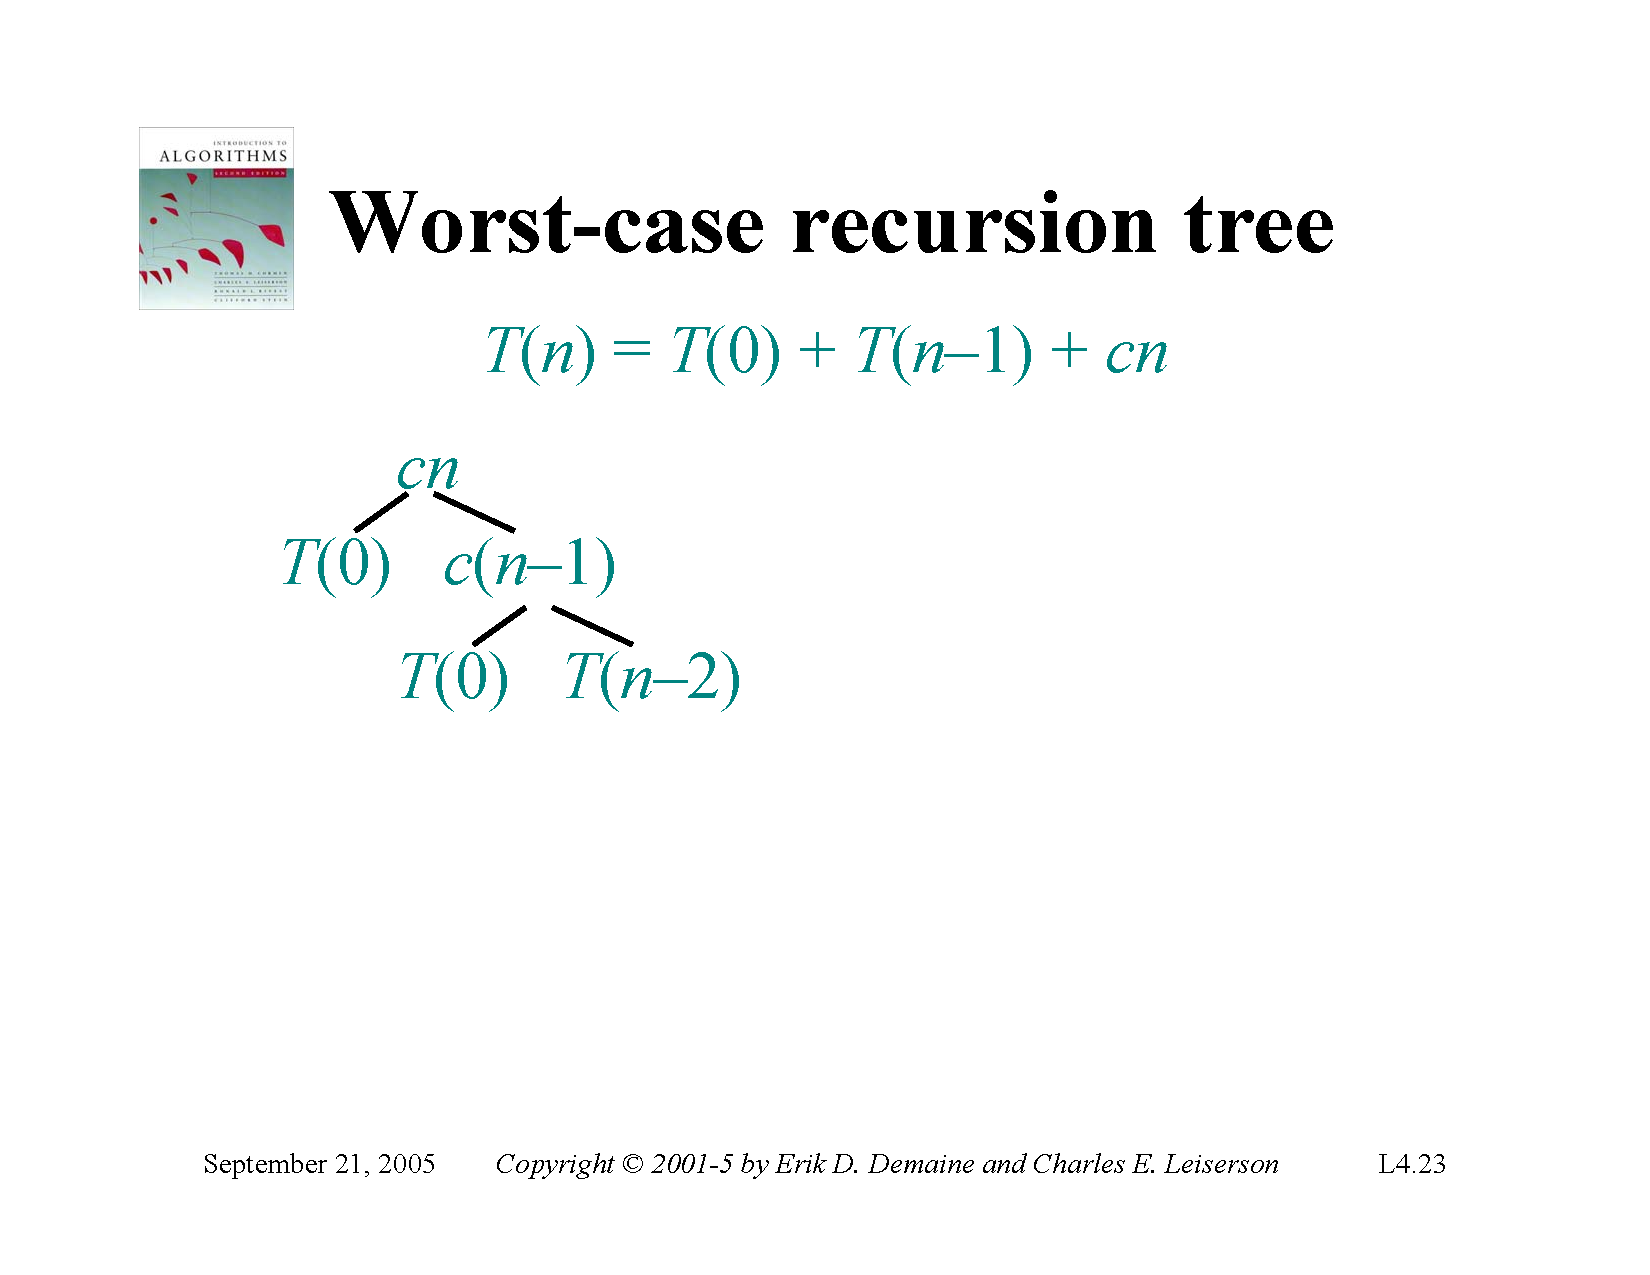
\includegraphics[width=\textwidth, trim={1.00cm 1.80cm 0.50cm 5.25cm}, clip]{pages/lec4_23}
\end{frame}
\begin{frame}{Worst-case Recursion Tree}
    \begin{equation*}
        \begin{split}
            T(n) =& T(0) + T(n - 1) + cn \\
        \end{split}
    \end{equation*}
    \centering
    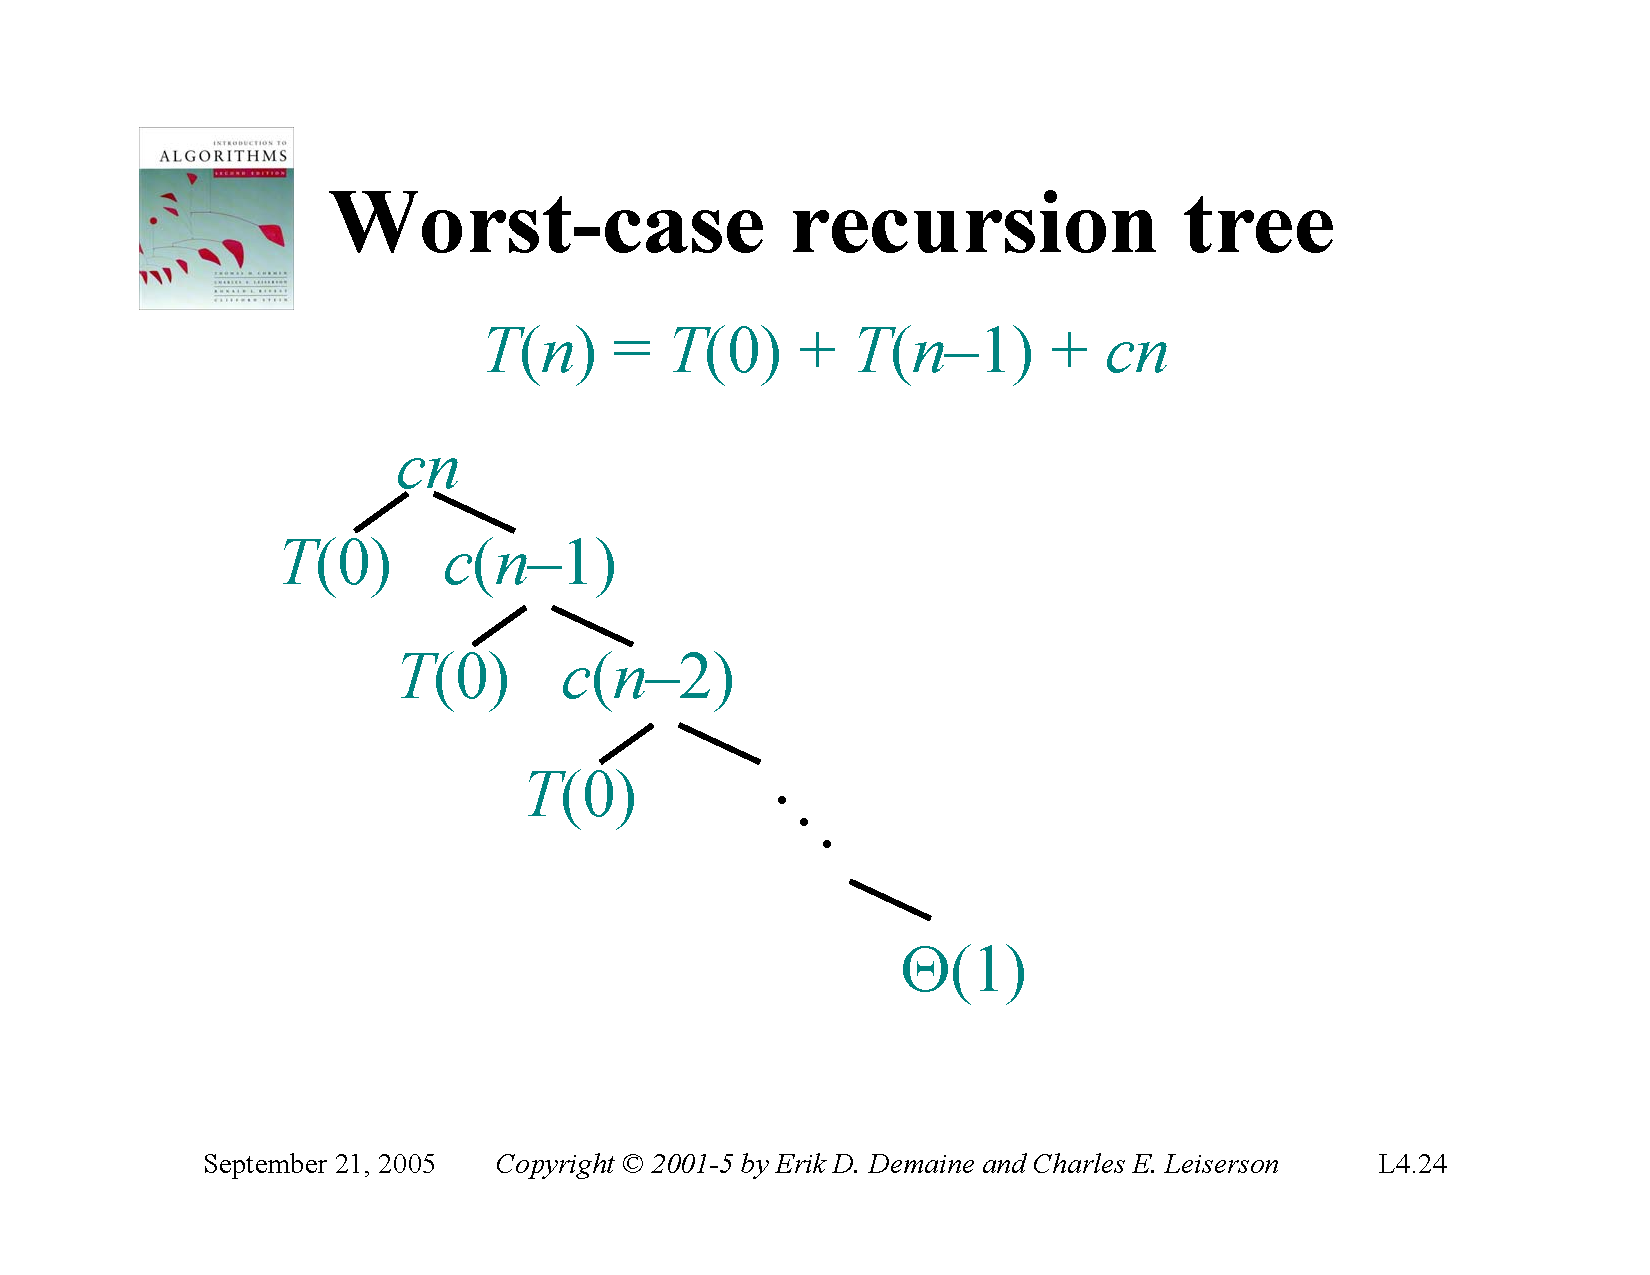
\includegraphics[width=\textwidth, trim={1.00cm 1.80cm 0.50cm 5.25cm}, clip]{pages/lec4_24}
\end{frame}
\begin{frame}{Worst-case Recursion Tree}
    \begin{equation*}
        \begin{split}
            T(n) =& T(0) + T(n - 1) + cn \\
        \end{split}
    \end{equation*}
    \centering
    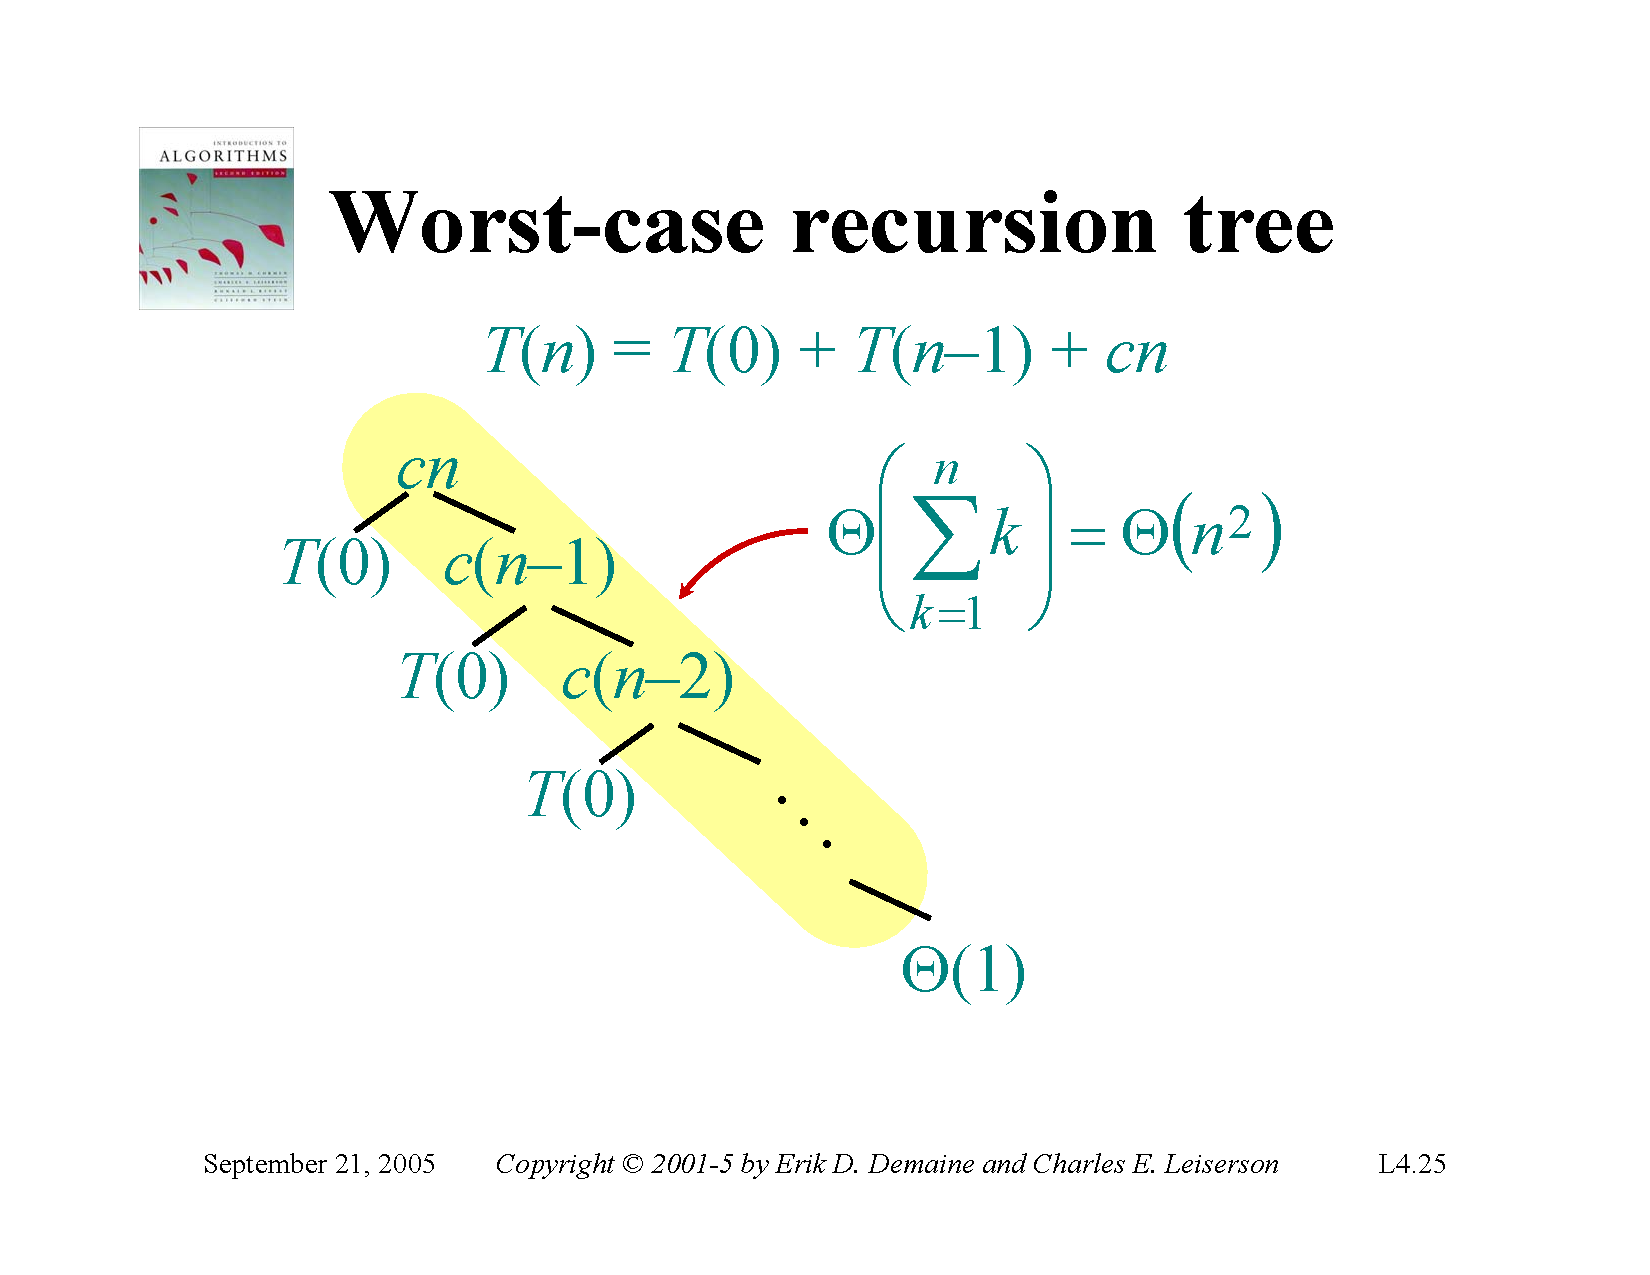
\includegraphics[width=\textwidth, trim={1.00cm 1.80cm 0.50cm 5.25cm}, clip]{pages/lec4_25}
\end{frame}
\begin{frame}{Worst-case Recursion Tree}
    \begin{equation*}
        \begin{split}
            T(n) =& T(0) + T(n - 1) + cn \\
        \end{split}
    \end{equation*}
    \centering
    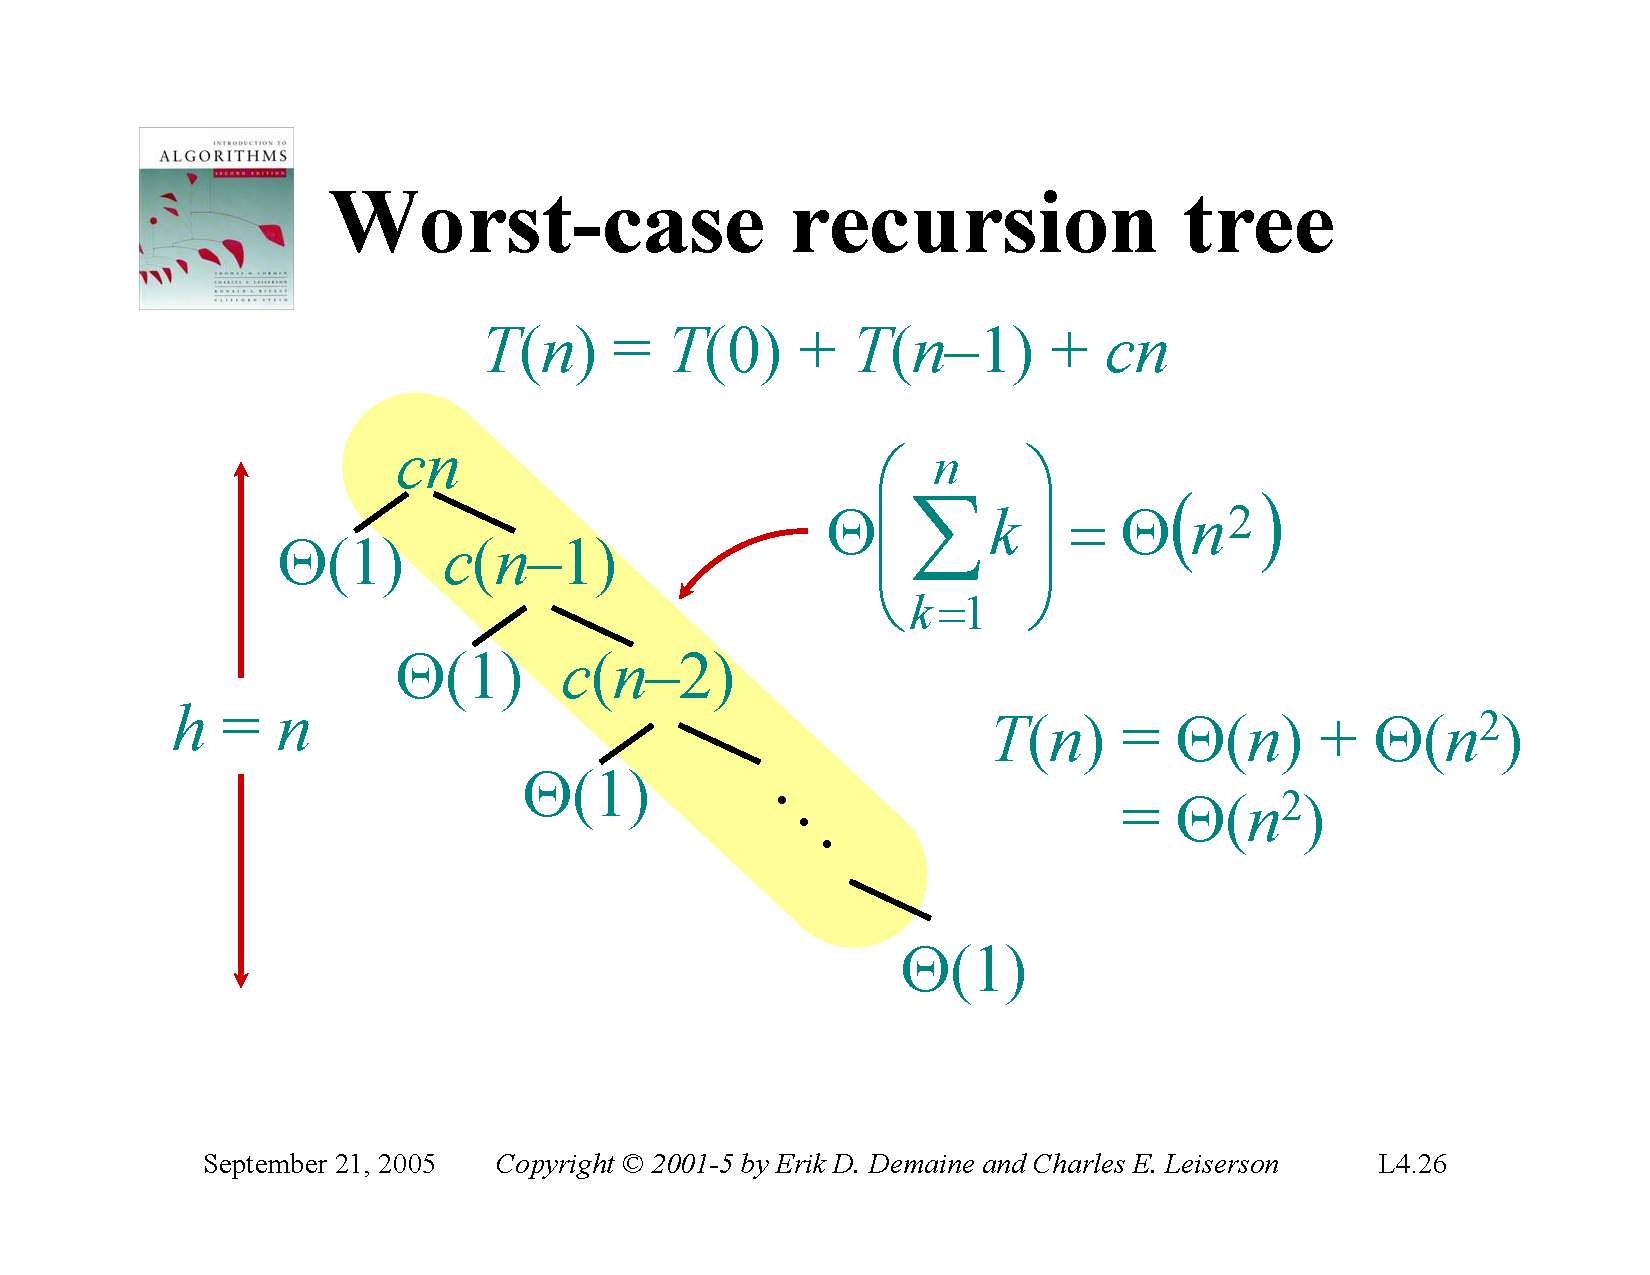
\includegraphics[width=\textwidth, trim={1.00cm 1.80cm 0.50cm 5.25cm}, clip]{pages/lec4_26}
\end{frame}

\section{Intuition}

\begin{frame}{Best-case Analysis}{For intuition only!}
    If we're lucky, \textsc{Partition} splits the array evenly:
    \begin{equation*}
        \begin{split}
            T(n) =& 2T\left(\frac{n}{2}\right) + \Theta(n) \\
                 =& \Theta(n \lg n) \text{\hspace{20mm} (same as merge-sort)} \\
        \end{split}
    \end{equation*}
    What if the split is always $\frac{1}{10}:\frac{9}{10}$?
    \begin{equation*}
        \begin{split}
            T(n) =& T\left(\frac{1}{10} n \right) + T\left(\frac{9}{10} n \right) + \Theta(n) \\
        \end{split}
    \end{equation*}
    What is the solution to this recurrence?
\end{frame}

\begin{frame}{Analysis of ``Almost-best'' Case}
    \centering
    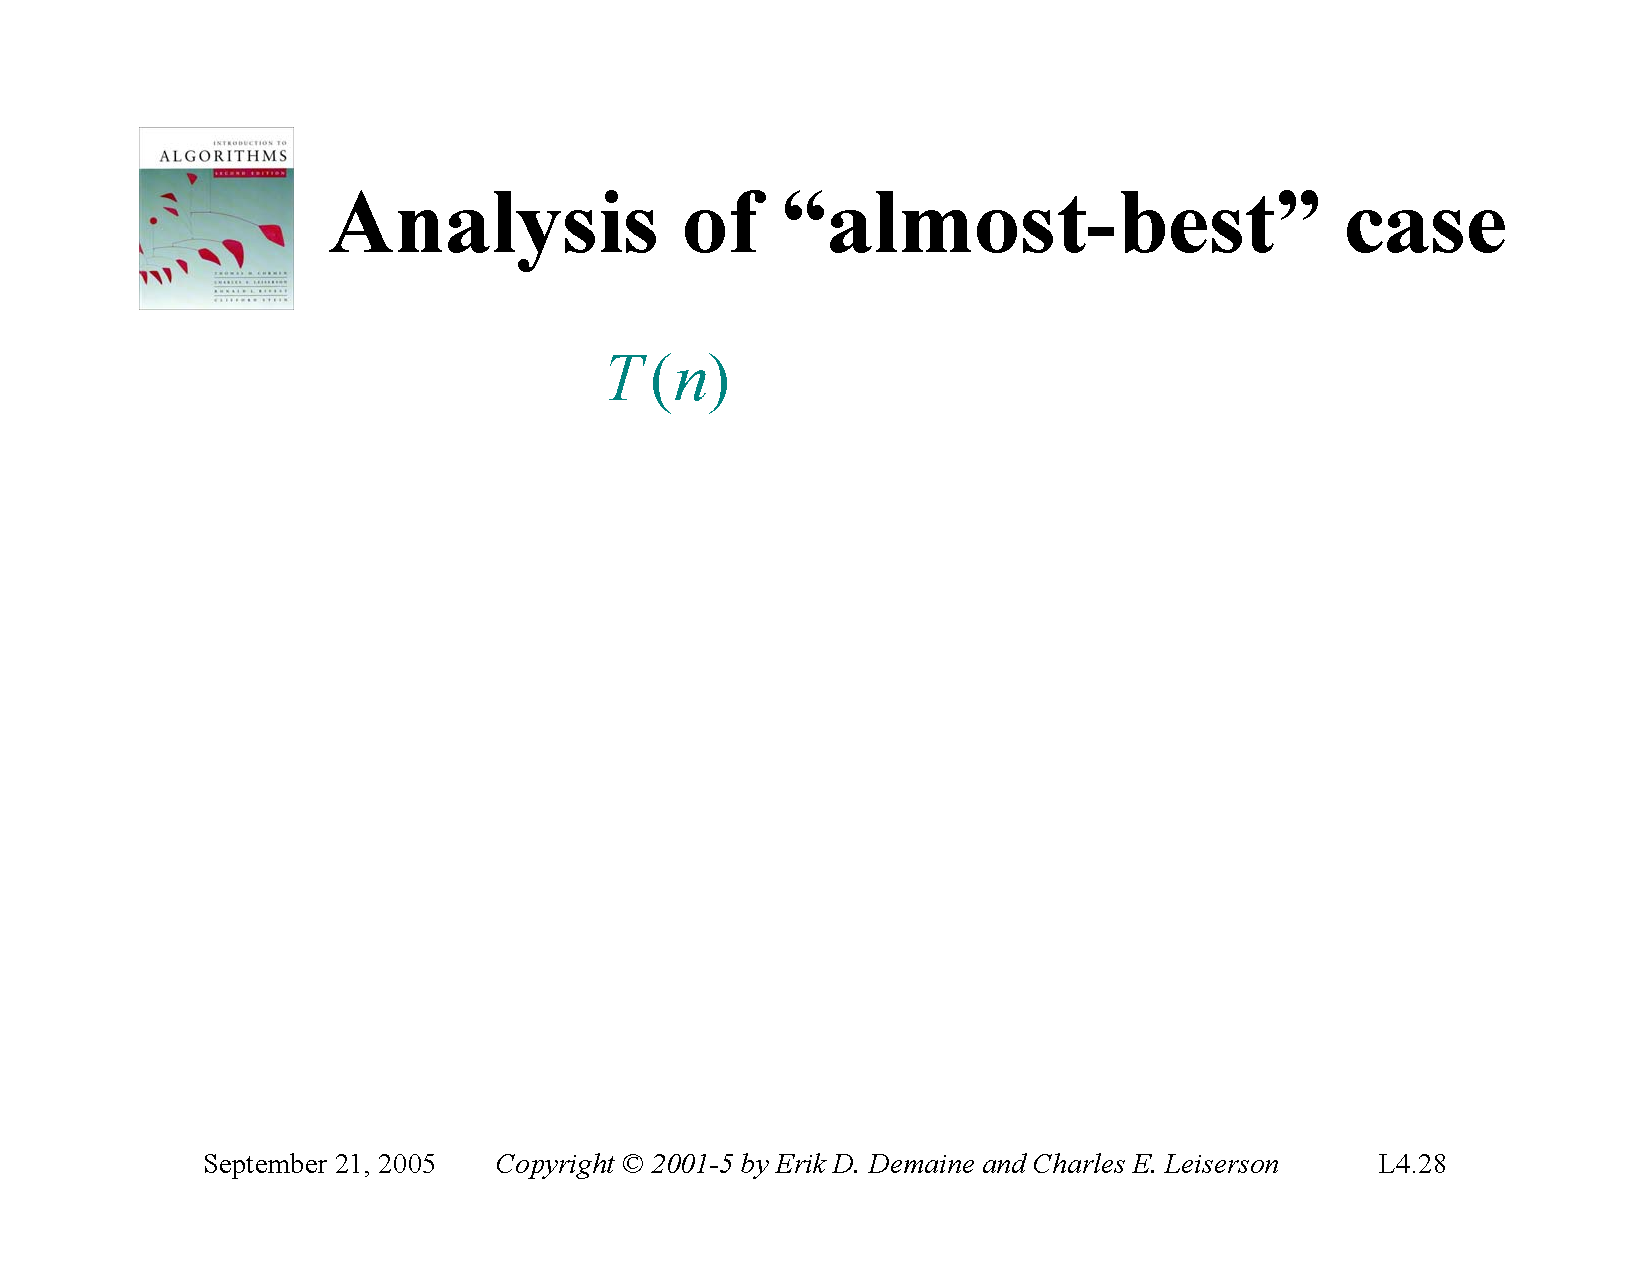
\includegraphics[width=\textwidth, trim={1.00cm 1.50cm 1.00cm 4.25cm}, clip]{pages/lec4_28}
\end{frame}
\begin{frame}{Analysis of ``Almost-best'' Case}
    \centering
    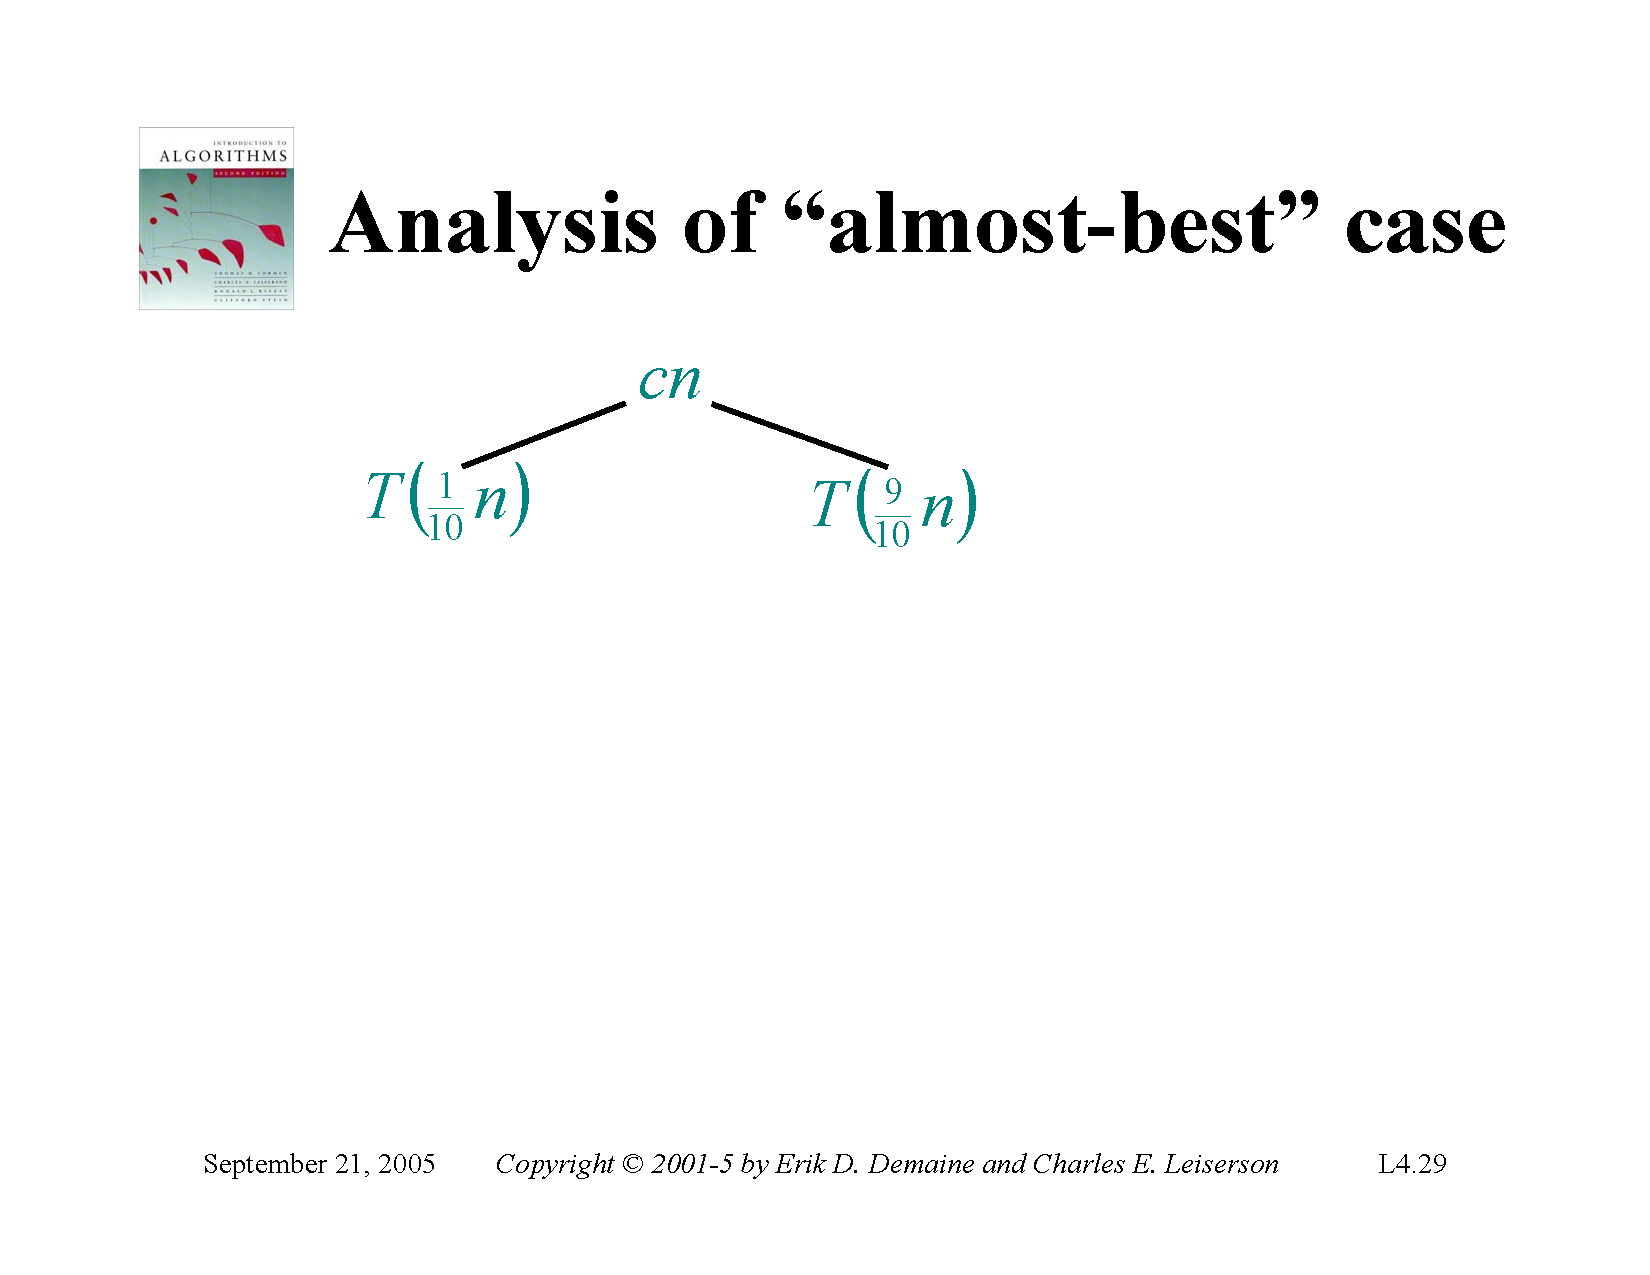
\includegraphics[width=\textwidth, trim={1.00cm 1.50cm 1.00cm 4.25cm}, clip]{pages/lec4_29}
\end{frame}
\begin{frame}{Analysis of ``Almost-best'' Case}
    \centering
    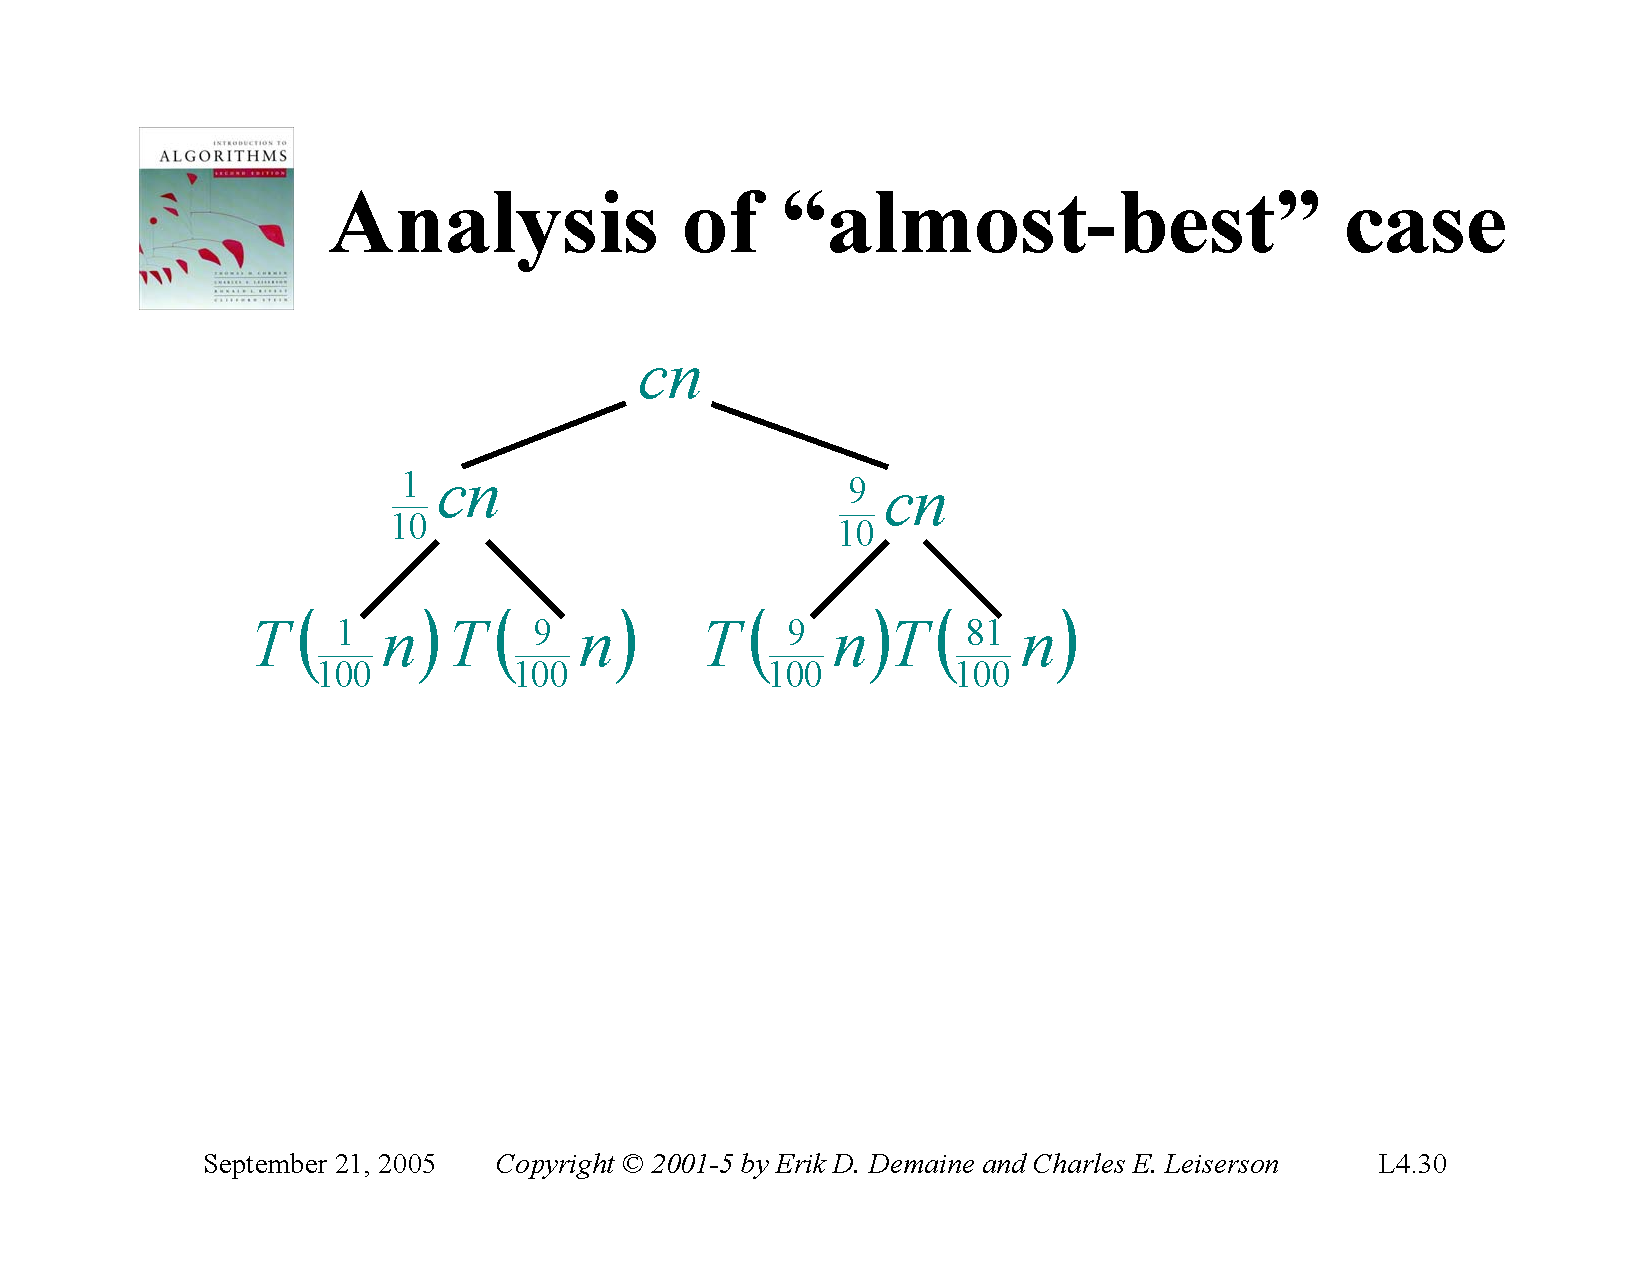
\includegraphics[width=\textwidth, trim={1.00cm 1.50cm 1.00cm 4.25cm}, clip]{pages/lec4_30}
\end{frame}
\begin{frame}{Analysis of ``Almost-best'' Case}
    \centering
    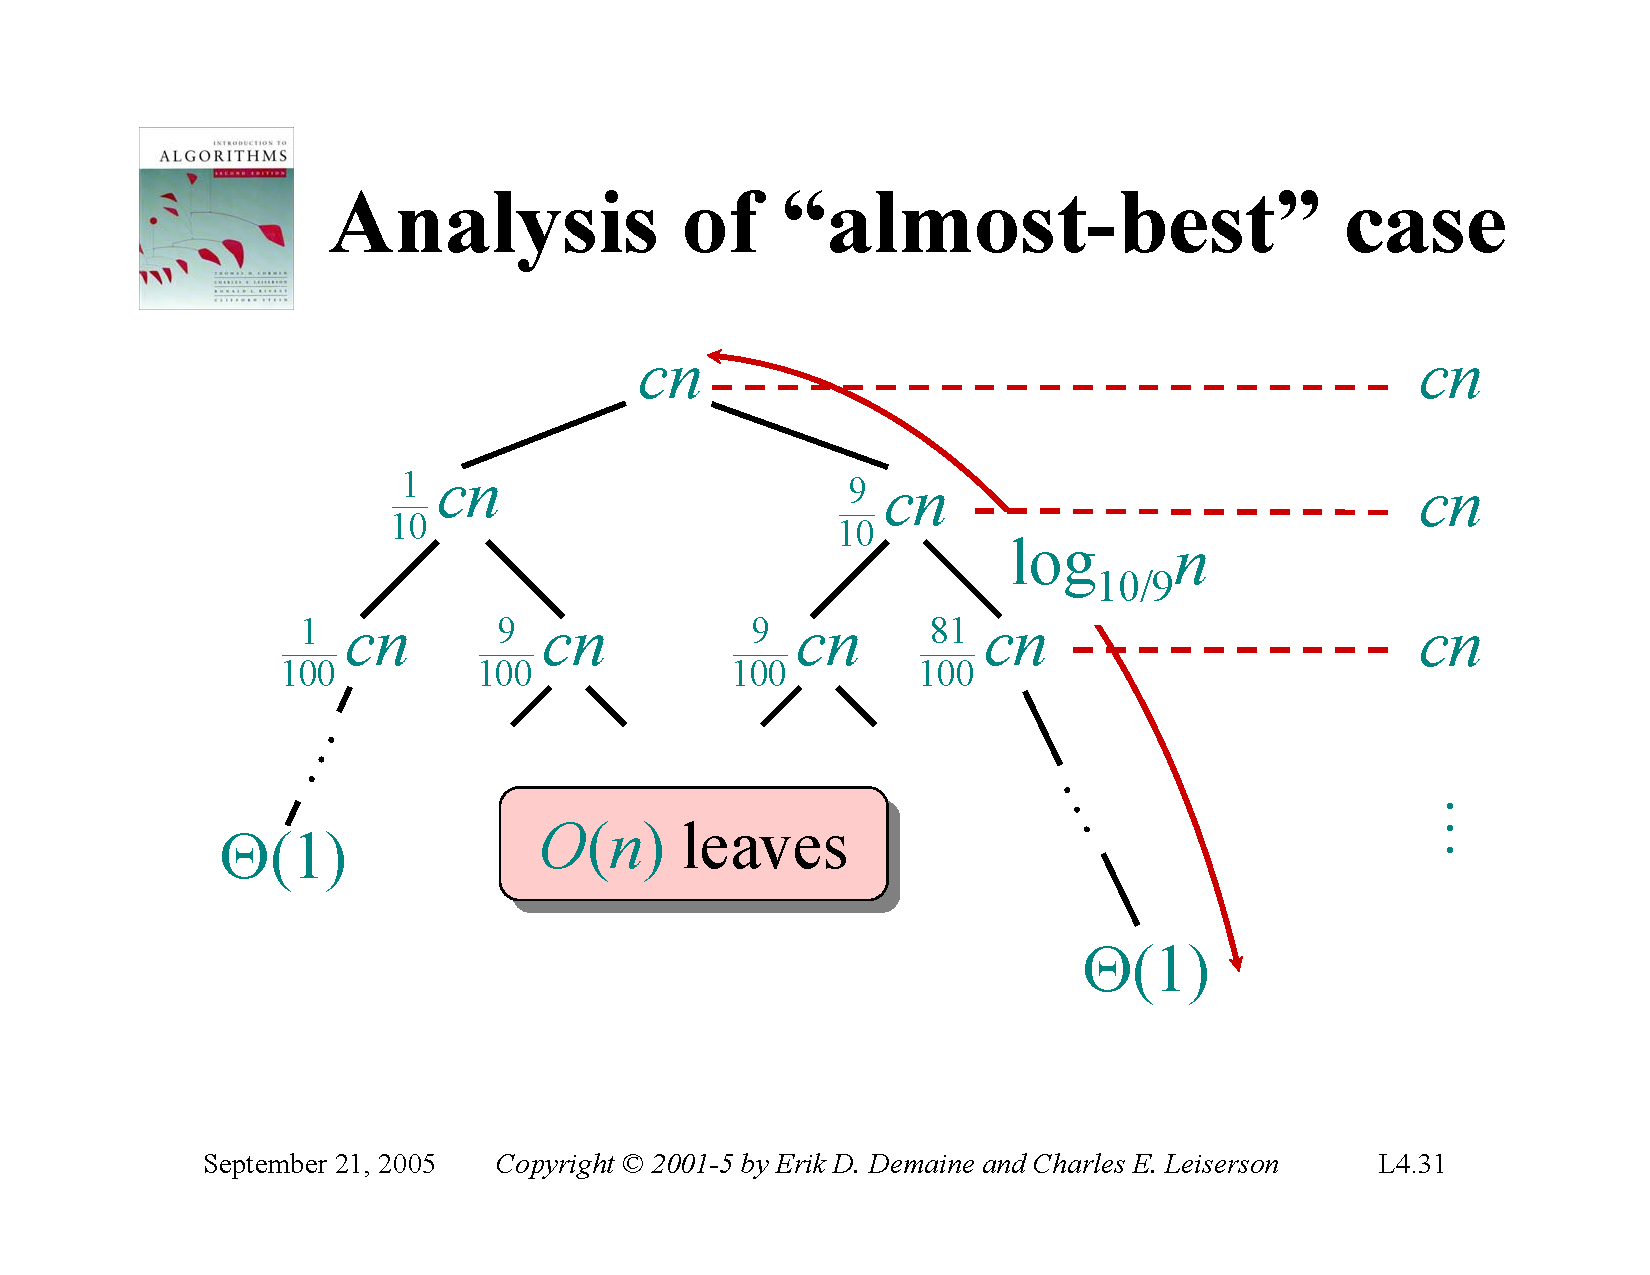
\includegraphics[width=\textwidth, trim={1.00cm 1.50cm 1.00cm 4.25cm}, clip]{pages/lec4_31}
\end{frame}
\begin{frame}{Analysis of ``Almost-best'' Case}
    \centering
    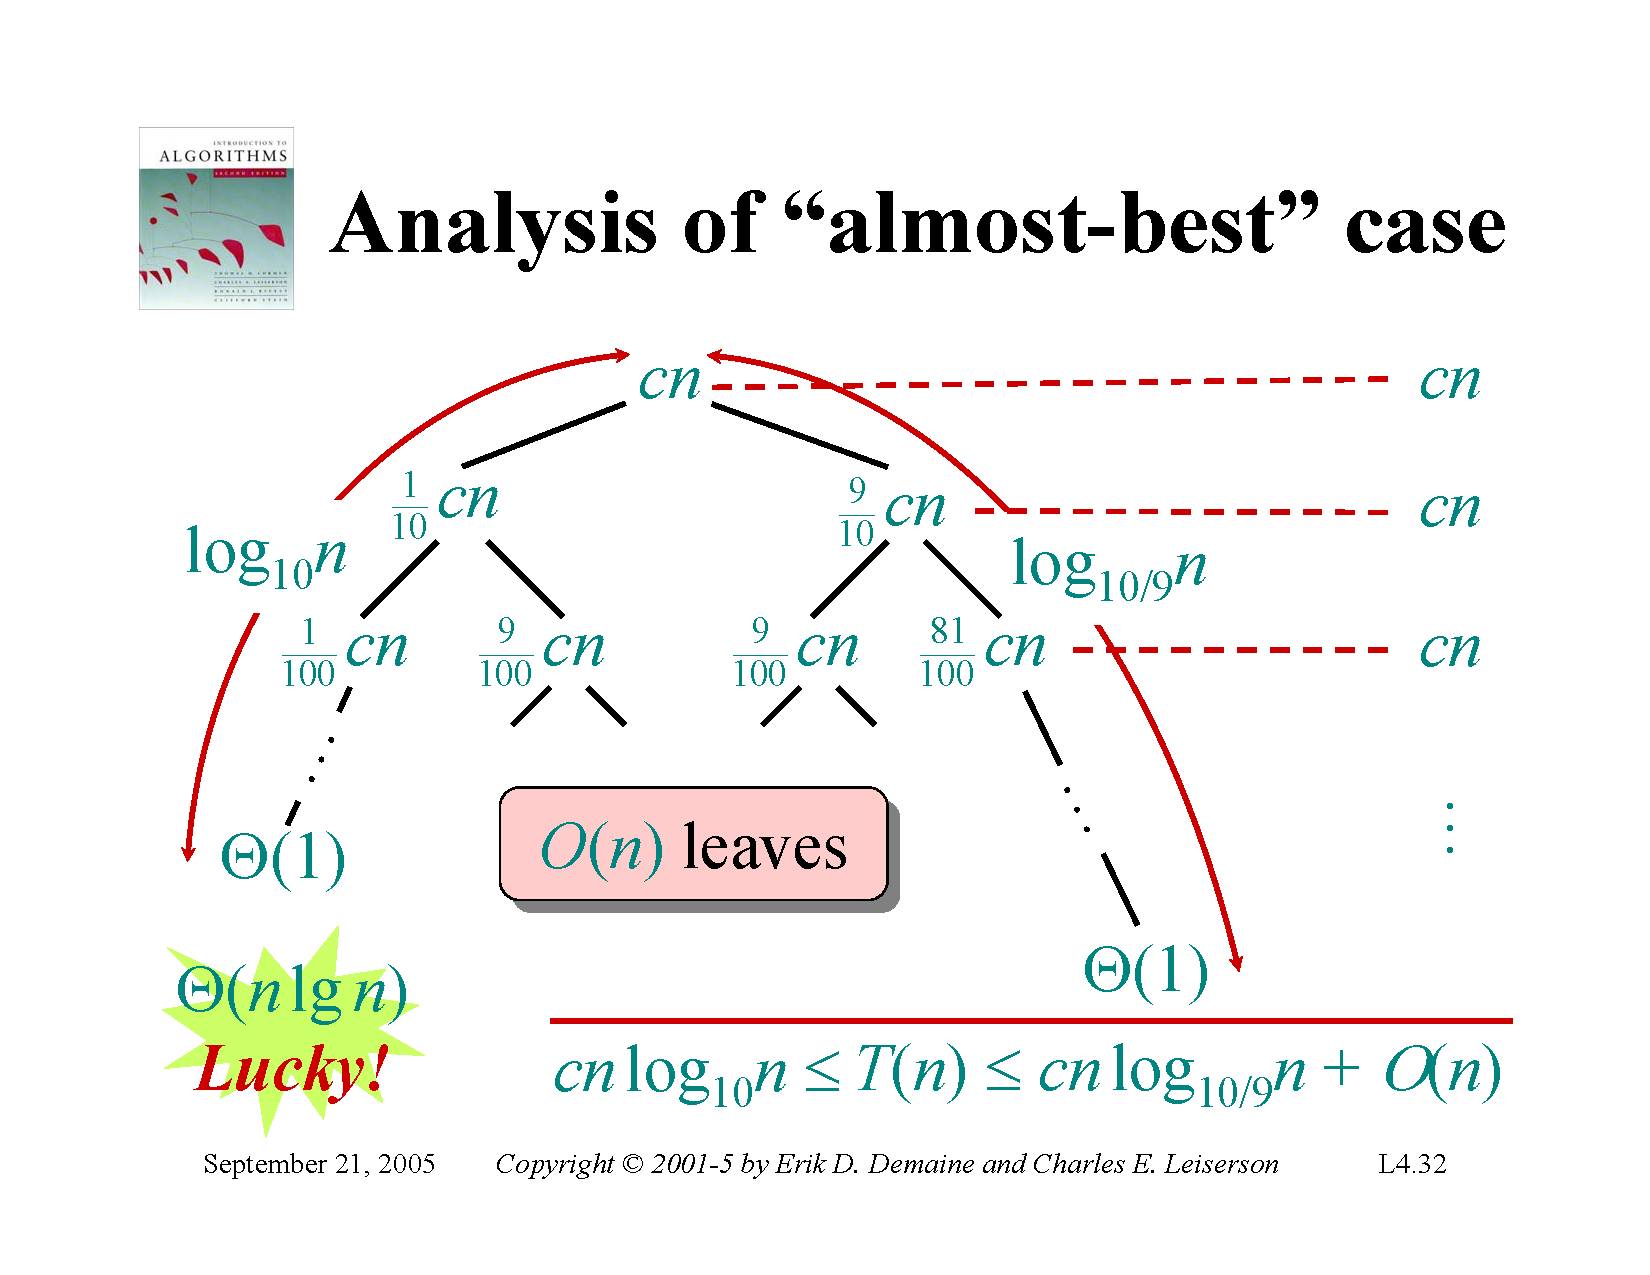
\includegraphics[width=\textwidth, trim={1.00cm 1.50cm 1.00cm 4.25cm}, clip]{pages/lec4_32}
\end{frame}

\begin{frame}{More Intuition}
    Suppose we alternate lucky, unlucky, lucky, unlucky, lucky, ...
    \begin{equation*}
        \begin{split}
            L(n) =& 2U\left(\frac{n}{2}\right) + \Theta(n) \text{\hspace{17mm} \textcolor{red}{\textit{luckcy}} } \\
            U(n) =& L\left(n - 1\right) + \Theta(n) \text{\hspace{15mm} \textcolor{red}{\textit{unluckcy}} } \\
        \end{split}
    \end{equation*}
    Solving:
    \begin{equation*}
        \begin{split}
            L(n) =& 2\left(L\left(\frac{n}{2} - 1 \right) + \Theta(\frac{n}{2})\right) + \Theta(n) \\
                 =& 2L\left(\frac{n}{2} - 1 \right) + \Theta(n) \\
                 =& \Theta(n \lg n) \text{\hspace{15mm} \textbf{\textcolor{red}{Lucky!}}}
        \end{split}
    \end{equation*}
    How can we make sure we are usually lucky?
\end{frame}

\section{Randomized Quicksort}

\begin{frame}{Randomized Quicksort}
    \begin{alertblock}{\textsc{Idea:}}
        Partition around a \textbf{random} element.
    \end{alertblock}
    \begin{itemize}
        \item Running time is independent of the input order.
        \item No assumptions need to be made about the input distribution.
        \item No specific input elicits the worst-case behavior.
        \item The worst case is determined only by the output of a random-number generator.
    \end{itemize}
\end{frame}

\section{Analysis}

\begin{frame}{Randomized Quicksort Analysis}
    Let $T(n) = $ the random variable for the running time of randomized quicksort on an input of size $n$, assuming random numbers are independent.
    $$
        \text{For } k = 0, 1, \ldots, n - 1\text{, define the \textcolor{red}{\textbf{indicator random variable}.}}
    $$

    $$
        X_k = \left\{
            \begin{array}{l l}
                \text{ 1 \text{\hspace{3mm}}} & \text{ if \textsc{Partition} generates a } k: n-k-1 split\text{,} \\
                \text{ 0 \text{\hspace{3mm}}} & \text{ otherwise.} \\
            \end{array}
        \right.
    $$
$E[X_k] = Pr\{X_k = 1\} = \frac{1}{n}$, since all splits are equally likely, assuming element are distinct.
\end{frame}

\begin{frame}{Analysis (Cont.)}
    $$
        T(n) = \left\{
            \begin{array}{l l}
                T(0) + T(n - 1) + \Theta(n) & \text{if } 0 : n - 1 \text{ split,} \\
                T(1) + T(n - 2) + \Theta(n) & \text{if } 1 : n - 2 \text{ split,} \\
                \text{\hspace{5mm}} \vdots & \\
                T(n - 1) + T(0) + \Theta(n) & \text{if } n - 1 : 0 \text{ split.} \\
            \end{array}
        \right.
    $$

    \vspace{10mm}
    \centering
    \Large
    $= \sum\limits_{k=0}^{n-1} X_k(T(k) + T(n - k - 1) + \Theta(n))$
\end{frame}

\begin{frame}{Calculating expectation}{Take expectations of both sides.}
    \begin{equation*}
        \begin{split}
E[T(n)] &= E\left[ \sum\limits_{k=0}^{n-1} X_k(T(k) + T(n - k - 1) + \Theta(n)) \right] \\
        \end{split}
    \end{equation*}
\end{frame}

\begin{frame}{Calculating expectation}{Linearity of expectation.}
    \begin{equation*}
        \begin{split}
E[T(n)] &= E\left[ \sum\limits_{k=0}^{n-1} X_k(T(k) + T(n - k - 1) + \Theta(n)) \right] \\
        &= \sum\limits_{k=0}^{n-1} E\left[ X_k(T(k) + T(n - k - 1) + \Theta(n)) \right] \\
        \end{split}
    \end{equation*}
\end{frame}

\begin{frame}{Calculating expectation}{Independence of $X_k$ from other random choices.}
    \begin{equation*}
        \begin{split}
E[T(n)] &= E\left[ \sum\limits_{k=0}^{n-1} X_k(T(k) + T(n - k - 1) + \Theta(n)) \right] \\
        &= \sum\limits_{k=0}^{n-1} E\left[ X_k(T(k) + T(n - k - 1) + \Theta(n)) \right] \\
        &= \sum\limits_{k=0}^{n-1} E[X_k] \cdot E[T(k) + T(n - k - 1) + \Theta(n)] \\
        \end{split}
    \end{equation*}
\end{frame}

\begin{frame}{Calculating expectation}{Linearity of expectation: $E[X_k] = \frac{1}{n}$.}
    \begin{equation*}
        \begin{split}
E[T(n)] &= E\left[ \sum\limits_{k=0}^{n-1} X_k(T(k) + T(n - k - 1) + \Theta(n)) \right] \\
        &= \sum\limits_{k=0}^{n-1} E\left[ X_k(T(k) + T(n - k - 1) + \Theta(n)) \right] \\
        &= \sum\limits_{k=0}^{n-1} E[X_k] \cdot E[T(k) + T(n - k - 1) + \Theta(n)] \\
        &= \frac{1}{n}\sum\limits_{k=0}^{n-1} E[T(k)] +
           \frac{1}{n}\sum\limits_{k=0}^{n-1} E[T(n - k - 1)] +
           \frac{1}{n}\sum\limits_{k=0}^{n-1} \Theta(n) \\
        \end{split}
    \end{equation*}
\end{frame}

\begin{frame}{Calculating expectation}{Summations have identical terms.}
    \begin{equation*}
        \begin{split}
E[T(n)] &= E\left[ \sum\limits_{k=0}^{n-1} X_k(T(k) + T(n - k - 1) + \Theta(n)) \right] \\
        &= \sum\limits_{k=0}^{n-1} E\left[ X_k(T(k) + T(n - k - 1) + \Theta(n)) \right] \\
        &= \sum\limits_{k=0}^{n-1} E[X_k] \cdot E[T(k) + T(n - k - 1) + \Theta(n)] \\
        &= \frac{1}{n}\sum\limits_{k=0}^{n-1} E[T(k)] +
           \frac{1}{n}\sum\limits_{k=0}^{n-1} E[T(n - k - 1)] +
           \frac{1}{n}\sum\limits_{k=0}^{n-1} \Theta(n) \\
        &= \frac{2}{n}\sum\limits_{k=0}^{n-1} E[T(k)] + \Theta(n) \\
        \end{split}
    \end{equation*}
\end{frame}

\begin{frame}{Hairy recurrence}
    \begin{equation*}
        \begin{split}
        E[T(n)] &= \frac{2}{n}\sum\limits_{k=2}^{n-1} E[T(k)] + \Theta(n) \\
        \end{split}
    \end{equation*}
    (The $k = 0$, $1$ terms can be absorbed in the $\Theta(n)$.)
    \begin{alertblock}{\textcolor{red}{\textbf{Prove:}}}
        $E[T(n)] \leq a n \lg n$ for constant $a > 0$.
    \end{alertblock}
    \begin{itemize}
        \item Choose a large enough so that $a n \lg n$ dominates $E[T(n)]$ for sufficiently small $n \geq 2$.
    \end{itemize}
    \begin{alertblock}{\textcolor{red}{\textbf{Use fact:}}}
        $\sum\limits_{k=2}^{n-1} k \lg k \leq \frac{1}{2} n^2 \lg n - \frac{1}{8} n^2$ (exercise).
    \end{alertblock}
\end{frame}

\begin{frame}{Substitution method}{Substitute inductive hypothesis.}
    \begin{equation*}
        \begin{split}
        E[T(n)] &\leq \frac{2}{n}\sum\limits_{k=2}^{n-1} a k \lg k + \Theta(n) \\
        \end{split}
    \end{equation*}
\end{frame}

\begin{frame}{Substitution method}{Use fact.}
    \begin{equation*}
        \begin{split}
        E[T(n)] &\leq \frac{2}{n}\sum\limits_{k=2}^{n-1} a k \lg k + \Theta(n) \\
                &\leq \frac{2a}{n} \left( \frac{1}{2}n^2 \lg n - \frac{1}{8}n^2 \right) + \Theta(n) \\
        \end{split}
    \end{equation*}
\end{frame}

\begin{frame}{Substitution method}
    \begin{equation*}
        \begin{split}
        E[T(n)] &\leq \frac{2}{n}\sum\limits_{k=2}^{n-1} a k \lg k + \Theta(n) \\
                &\leq \frac{2a}{n} \left( \frac{1}{2}n^2 \lg n - \frac{1}{8}n^2 \right) + \Theta(n) \\
                &= a n \lg n - \left( \frac{an}{4} - \Theta(n) \right) \\
                &\leq a n \lg n \text{,} \\
                &\text{\hspace{10mm} if $a$ is chosen large enough so that} \\
                &\text{\hspace{10mm} $\frac{an}{4}$ dominates the $\Theta(n)$.}
        \end{split}
    \end{equation*}
\end{frame}

\begin{frame}{Quicksort in practice}
    \begin{itemize}
        \item Quicksort is a great general-purpose sorting algorithm.
        \item Quicksort is typically over twice as fast as merge sort.
        \item Quicksort can benefit substantially from \textcolor{red}{\textbf{code tuning}}.
        \item Quicksort behaves well even with caching and virtual memory.
    \end{itemize}
\end{frame}

\begin{frame}{}
    \centering
    \Huge End of Lecture 4.
\end{frame}

\section*{Takeaways}

% Tim Duncan's Top 5 Fundamental Takeaways of the Today's Class
\begin{frame}{TDT5FTOTTC}
    \centering
    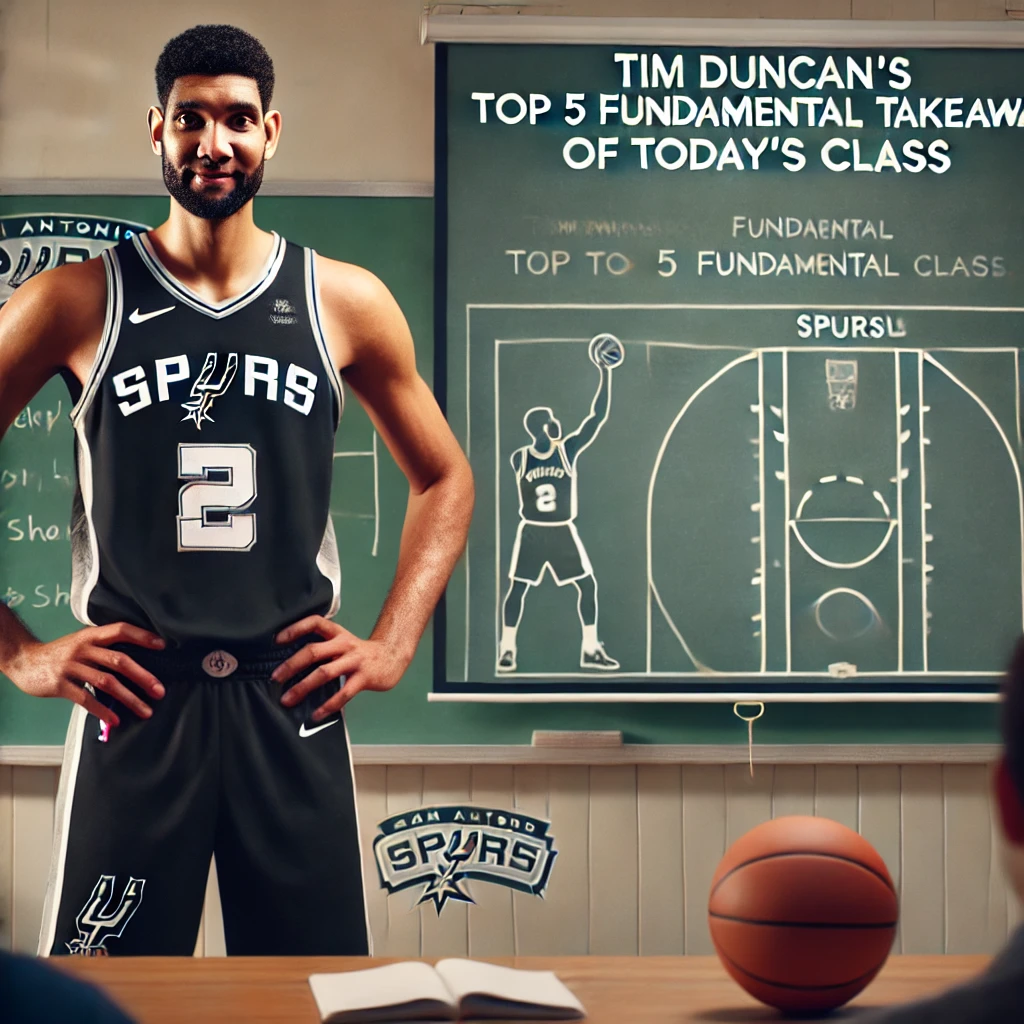
\includegraphics[width=0.75\textwidth]{figures/tim.png}
\end{frame}

\begin{frame}{Top 5 Fundamental Takeaways}
    \small
    \begin{enumerate} \pause
        \item[5] \textbf{Quicksort is a Divide-and-Conquer Algorithm} – It recursively partitions an array around a pivot and sorts the subarrays efficiently.\pause

        \item[4] \textbf{Partitioning is the Core of Quicksort} – The partitioning step ensures elements are correctly placed around the pivot in $O(n)$ time.\pause

        \item[3] \textbf{Best-case and Worst-case Analysis} – Quicksort runs in $O(n \log n)$ in the best case but can degrade to $O(n^2)$ if poorly partitioned.\pause

        \item[2] \textbf{Randomized Quicksort Helps Avoid Worst-case Behavior} – Choosing a random pivot prevents consistently bad splits and ensures an expected $O(n \log n)$ runtime.\pause

        \item[1] \textbf{Quicksort is Highly Efficient in Practice} – It outperforms merge sort in most cases and benefits from hardware optimizations.

    \end{enumerate}
\end{frame}

\begin{frame}{Introduction to Algorithms}
    \centering
    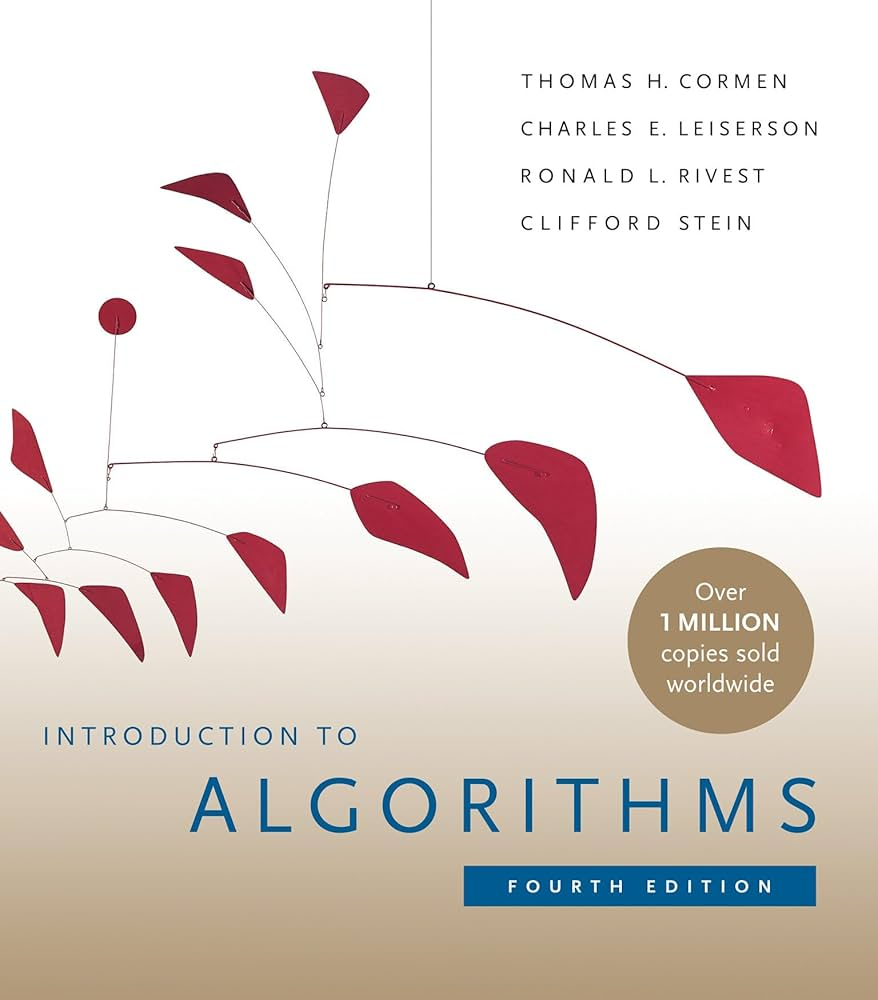
\includegraphics[width=0.45\textwidth]{figures/book_cover.jpg} \\
    \vspace{5mm}{
        \tiny
        Content has been extracted from \textit{Introduction to Algorithms}, Fourth Edition, by Cormen, Leiserson, Rivest, and Stein. MIT Press. 2022.\\
        Visit \url{https://mitpress.mit.edu/9780262046305/introduction-to-algorithms/}.\\
        Original slides from \textit{Introduction to Algorithms 6.046J/18.401J}, Fall 2005 Class by Prof. Charles Leiserson and Prof. Erik Demaine. MIT OpenCourseWare Initiative available at \url{https://ocw.mit.edu/courses/6-046j-introduction-to-algorithms-sma-5503-fall-2005/}.\\
    }
\end{frame}

\end{document}
